\documentclass{article}
\usepackage{iclr2027_conference,times}
\usepackage{amsmath,amssymb,booktabs,graphicx,etoolbox,array}
\usepackage{url}
\usepackage[hidelinks]{hyperref}
\hypersetup{pdftitle={Does Stored-Token Uncertainty Improve Trajectory Repair? A Controlled HotpotQA Study},pdfauthor={}}
% Keep words intact across page breaks, especially around floating results.
\brokenpenalty=10000

\title{Does Stored-Token Uncertainty\\Improve Trajectory Repair?\\A Controlled HotpotQA Study}
\author{Anonymous authors}
% This local working copy has not been submitted; leave the official style file intact.
\makeatletter
\patchcmd{\@maketitle}{Paper under double-blind review}{Working draft; not submitted}{}
  {\PackageError{agent-repair}{Working-draft label patch failed}{Check the title macro.}}
\makeatother
% Generated by scripts/build_iclr_draft.py; Main* macros are audited HotpotQA results.
\newcommand{\HotpotFailed}{226}
\newcommand{\HotpotJudge}{10.9}
\newcommand{\HotpotBacktrack}{12.4}
\newcommand{\HotpotRestart}{14.2}
\newcommand{\HotpotBestUnc}{12.8}
\newcommand{\HotpotGain}{1.5}
\newcommand{\MusiqueFailed}{425}
\newcommand{\MusiqueJudge}{4.9}
\newcommand{\MusiqueBacktrack}{5.6}
\newcommand{\MusiqueRestart}{5.9}
\newcommand{\MusiqueBestUnc}{5.6}
\newcommand{\MusiqueGain}{0.7}
\newcommand{\WikiFailed}{203}
\newcommand{\WikiJudge}{10.0}
\newcommand{\WikiBacktrack}{22.0}
\newcommand{\WikiRestart}{21.2}
\newcommand{\WikiBestUnc}{25.5}
\newcommand{\WikiGain}{12.0}
\newcommand{\TotalFailed}{854}
\newcommand{\MainInitial}{250}
\newcommand{\MainFailed}{113}
\newcommand{\MainUniqueRepairs}{1,058}
\newcommand{\MainSeedRows}{2,034}
\newcommand{\MainTreatmentRate}{9.73}
\newcommand{\MainRestartRate}{11.21}
\newcommand{\MainRestartDelta}{-1.47}
\newcommand{\MainRestartLow}{-4.13}
\newcommand{\MainRestartHigh}{+0.88}
\newcommand{\MainEstimatedUSD}{9.16}
\newcommand{\MainObservations}{8,552}
\newcommand{\MainPrefixes}{1,742}
\newcommand{\MainTrajectories}{1,308}
\newcommand{\ReviewActiveQuestions}{43}
\newcommand{\ReviewActiveDelta}{-3.88}
\newcommand{\ReviewActiveLow}{-10.85}
\newcommand{\ReviewActiveHigh}{+2.33}
\newcommand{\ReviewPromptIncrease}{29.5}
\newcommand{\ReviewBudgetStops}{103}
\newcommand{\ReviewStepStops}{65}
\newcommand{\ReviewBudgetStopRate}{30.38}
\newcommand{\ReviewWholeSuccess}{59.20}
\newcommand{\ReviewWholeRestartSuccess}{59.87}

% Working draft. The evidence and rerun requirements are recorded in
% ../docs/iclr2027_readiness.md. Do not submit before those checks are complete.

\begin{document}
\maketitle
\fancyhead[L]{Working draft: audited HotpotQA study}

\begin{abstract}
When a language model agent fails, recovery can preserve a trajectory prefix
and regenerate its suffix, or restart from the original task. We test whether
stored-token uncertainty helps select a recovery origin beyond simple
positional choices in a ReAct-style agent. A controlled experiment with
Qwen2.5-32B-Instruct-AWQ freezes \MainInitial{} HotpotQA questions before
inference. Its \MainFailed{} initial failures receive six repair conditions
and three seeds under matched retry hints, generated-token caps and new-step
allowances. The prespecified perplexity/argmax policy with two-step
backtracking achieves \MainTreatmentRate\% repair success, versus
\MainRestartRate\% for full restart: a difference of \MainRestartDelta{}
percentage points, with a question-level 95\% bootstrap interval from
\MainRestartLow{} to \MainRestartHigh{}. Its success rate equals the
position-matched random control; none of the four prespecified comparisons
shows a clear advantage after Holm correction. Exploratory trace diagnostics
show that the treatment differs from restart on only \ReviewActiveQuestions{}
failed questions and uses \ReviewPromptIncrease\% more prompt tokens, with
similar generated-token use. All \MainUniqueRepairs{} unique repair executions
pass independent replay, scoring and allowance audits. Historical exclusion
IDs are reconstructed, with the original full pool comparison unavailable.
A separate 250-question cohort compares restart, uncertainty, and same-model
diagnosis/replay at three allowances, with 2,079 additional unique repairs.
Uncertainty again shows no clear advantage in six Holm-adjusted comparisons.
These results do not establish equivalence or an advantage under equal total compute.
\end{abstract}

\section{Introduction}
ReAct agents interleave reasoning, tool calls, and observations
\citep{yao2023react}; a failed answer can reflect mistakes at several points.
Recovery must decide both what to change and how much context to retain.
Restart discards potentially useful work. Suffix regeneration preserves
that work but constrains recovery to the retained reasoning and observations.

Error attribution and recovery need not have the same objective. Attribution
asks which step is erroneous, whereas recovery asks where a new rollout is
most likely to succeed at an acceptable cost. A judge may identify an
incorrect conclusion that is downstream of incomplete evidence gathering.
Conversely, a locally uncertain action can be useful exploration. Neither
uncertainty nor agreement with an error annotation directly establishes
the value of intervening at that step.

We examine this distinction using a common execution loop for targeted
regeneration and restart. The historical framework crosses five signals
with six origin-selection rules and uses a larger model for privileged
reference diagnostics. The completed six-condition study freezes one stored-token
policy and evaluates six conditions under matched recovery allowances on
HotpotQA. It uses no judge or outcome-based policy search. Reference annotations are not treated
as infallible causal labels. Prior work already studies intervention-based
debugging, localized QA repair with prefix reuse, and repair versus
resampling \citep{ma2026dover,jiao2026doctor,luan2026symtrace}.
The unresolved question here is whether stored-token uncertainty adds
origin-selection value beyond position alone, without a separate diagnosis
model, in a fixed tool environment. Neither prefix reuse nor the distinction
between attribution and recovery is claimed as new.

The evidence does not support a universal short-trajectory repair versus
long-trajectory restart rule: evidence quality, error types, dataset, and
budget can influence the ordering. We focus on three contributions:
\begin{enumerate}
\item A prespecified six-condition HotpotQA comparison with question-level
      paired inference, including a development-fitted position control
      and a no-backtracking ablation; no clear uncertainty advantage is observed.
      A separate 250-question follow-up adds a same-model diagnosis/replay
      adaptation at three recovery-token allowances, also without a clear
      uncertainty advantage.
\item An exploratory decomposition of shared executions and observed
      resource use, which exposes the limited number of distinct interventions
      and separates output-token allowances from repeated prompt processing.
\item Audited replay, reference scoring, complete trial coverage and frozen
      inputs supporting reproduction of the controlled comparison. Older
      three-dataset summaries are retained as separate historical context.
\end{enumerate}

\section{Related Work}
\paragraph{Agent recovery and self-correction.}
Reflexion uses verbal feedback from previous episodes to inform subsequent
attempts \citep{shinn2023reflexion}, while Self-Refine iteratively improves
outputs using generated feedback \citep{madaan2023selfrefine}.
\citet{huang2024large} document limitations of intrinsic reasoning
self-correction without external feedback. Our benchmark provides an
external correctness gate that selects failed attempts. Conditional on
that gate, we study suffix origins, not online failure detection.

\paragraph{Localized repair and replay.}
ReAgent uses local and global rollback in multi-agent QA
\citep{xinjie2025reagent}. Doctor-RAG diagnoses failure type and location,
then reuses prefixes and evidence for local repair on HotpotQA, MuSiQue,
and 2WikiMultiHopQA \citep{jiao2026doctor}. This is direct task-level
overlap, although its trained diagnoser, retrieval setting, and repair
operators differ from our stored-token selector. DoVer evaluates
intervention-driven debugging through task recovery \citep{ma2026dover}.
SymTrace reconstructs recorded prefixes to examine repair versus
resampling \citep{luan2026symtrace}; AgentRewind coordinates context and
workspace rollback with memory of prior attempts \citep{zhuang2026agentrewind}.
Our offline tool replay is narrower than general environment rollback.

\paragraph{Step evaluation and failure attribution.}
Process supervision evaluates intermediate reasoning \citep{lightman2024lets},
and Who\&When studies multi-agent failure locations \citep{zhang2025which}.
AgentRx uses executable constraints and violation logs to support diagnosis
\citep{barke2026agentrx}. REFLECT, Causal Agent Replay, and CausalFlow
study interventions for attribution or repair
\citep{lin2026reflect,shah2026causal,bonagiri2026causalflow}.
AgenticRAG-FP injects faults and re-executes downstream reasoning to test
attribution against known interventions \citep{pothuru2026failures}.
Our naturally failed traces lack such intervention-grounded causal labels.

\paragraph{Uncertainty signals.}
Self-consistency aggregates sampled reasoning outputs
\citep{wang2023selfconsistency}, and verbalized confidence can provide
useful calibration information \citep{tian2023just}.
ERGO already uses entropy changes for conversation resets
\citep{khalid2025ergo}. The archived framework includes action-level signals
and stored-token statistics; the controlled study tests perplexity alone,
without assuming calibration as error probabilities.
Appendix~\ref{app:related} specifies the closest comparisons and information
differences. No head-to-head advantage over these methods is established.

\section{Problem and Evaluation Targets}
\label{sec:problem}
An instance consists of a question $x$, an offline document collection
$D_x$, and a reference answer $y$. An agent produces a trajectory
$\tau=(s_0,\ldots,s_{T-1})$. Each step contains generated reasoning, a
tool action, its argument, and the returned observation. The available
actions are \texttt{search}, \texttt{lookup}, and \texttt{finish}.

\paragraph{Failure gate.}
The implemented QA success criterion accepts an answer when its normalized
exact match is one or its token F1 is at least $0.5$. This threshold is a
study-specific recovery criterion, not the official aggregate metric for
every benchmark. Only trajectories that fail this gate enter repair.
Evaluation therefore estimates recovery conditional on a known benchmark
failure; the reference answer is not available to an ordinary deployed
failure detector.

\paragraph{Repair origin.}
For an origin $k\in\{0,\ldots,T-1\}$, targeted repair retains
$s_0,\ldots,s_{k-1}$ and generates a new suffix. Tool calls in the retained
prefix are replayed to restore the environment state. Full restart uses
$k=0$. With backtracking offset $b$, the effective origin is
\begin{equation}
  k' = \max(0,k-b).
\end{equation}
Backtracking can make several nominal strategies share the same origin,
and can turn targeted repair into a restart. Consequently, strategy counts
are not counts of independent interventions.

\paragraph{Reference annotations.}
Let $k_J$ denote the earliest erroneous step identified by a language model
judge. Agreement with $k_J$ measures reference-label localization. It is
distinct from the origin that maximizes expected repair success,
\begin{equation}
  k^*(\tau,B)=\arg\max_k
  \Pr\!\left[\operatorname{correct}(\operatorname{repair}(\tau,k,B))\right].
\end{equation}
The latter depends on the agent, retained context, recovery prompt, and
budget $B$, and is not observed merely by asking a judge to label a trace.

\paragraph{Success across seeds.}
For failed question $q$, strategy $a$, and generation seed $r$, write the
binary repair outcome as $Y_{qar}$. Our primary descriptive statistic is
\begin{equation}
  \widehat{R}_a = \frac{1}{N}\sum_{q=1}^{N}
                 \frac{1}{S_q}\sum_{r=1}^{S_q}Y_{qar}.
  \label{eq:success}
\end{equation}
Each question receives equal weight. Thresholding each question's mean
success to obtain a majority-over-seeds outcome measures repeatability,
not the success rate of one sampled repair, and must be reported separately.

\section{Uncertainty-Guided Regeneration}
\subsection{Prespecified Stored-Token Policy}
The controlled study uses step perplexity from stored sampled-token log
probabilities. For log probability $\ell_{it}$ of generated token $t$ in
step $i$, define
\begin{equation}
 U_i^{\mathrm{ppl}}=\exp\!\left(\min\left\{20,
                  -\frac{1}{n_i}\sum_{t=1}^{n_i}\ell_{it}\right\}\right).
\end{equation}
The policy selects the highest finite step score, breaking ties toward
the earlier step, then subtracts two trajectory indices and clamps at zero.
No additional uncertainty-acquisition model calls are required. Unusable
measurements are skipped; an empty usable profile falls back to origin zero.
This stored-token measure requires no additional sampled rollouts or diagnosis
model. The policy was prespecified before main-study outcomes, rather than
chosen as the best-performing development or test variant; this is not an
evaluation of the best possible uncertainty estimator.

The historical framework also evaluates entropy, sampled-token probability
complement, action disagreement and verbalized uncertainty with several
localization rules. Appendix~\ref{app:signals} preserves their definitions.
Those historical configurations are not additional conditions in the
controlled experiment.

\subsection{Interventions and Information Access}
Full restart discards the failed context; targeted policies retain a prefix.
All six controlled conditions receive the same generic retry hint. The
uncertainty selector can inspect the complete failed
trace's uncertainty profile, but receives no answer or supporting-fact
labels. The recovery model sees only the question, retained prefix, and
generic hint; discarded suffix observations are not inserted into its
prompt. The same offline collection remains searchable. This is post-hoc
selection after failure, not a policy that predicts the origin online.
Judge-targeted and reference-informed repair belong only to the archived
experiments. Their privileged information and unmatched historical restart
hint are documented separately in Appendix~\ref{app:implementation}.

\subsection{Budget Scope}
The controlled repair cap is the original failed trajectory's generated-token
count. Each request is bounded by the remaining cap, with at most eight new
steps and 512 generated tokens per step. Retained steps do not consume new-step
opportunities. The historical runner instead counted retained steps toward
its eight-step limit and could overshoot its token cap during a final request.
Its outcomes remain separate. Even the corrected allowances do not equalize
realized tokens, prompt processing, latency or FLOPs; these require additional
cost measurements.

\section{Completed HotpotQA Study}
\label{sec:evidence}
\subsection{Model, Cohort and Historical Exclusions}
We evaluated Qwen2.5-32B-Instruct-AWQ on \MainInitial{} HotpotQA questions
\citep{yang2018hotpotqa} using the supplied distractor-context paragraphs:
248 questions have ten paragraphs, one has two, and one has six.
The offline \texttt{search} tool uses exact, substring and fuzzy title
matching and returns the first five sentences; \texttt{lookup} advances
through matching sentences in the current paragraph. Model
and tokenizer were pinned to one snapshot (Appendix~\ref{app:completion}).
Initial generation was greedy; repairs used temperature $0.7$ and seeds
$0,1,2$. Five ordered batches of 50 completed on September 12, 2026. There
was no adaptive sample-size change or policy selection after new outcomes.

The cohort was sampled uniformly without replacement from 6,856 sorted
eligible IDs using seed 20260912, giving 196 bridge and 54 comparison
questions. We excluded 549 distinct IDs: the union of a reconstructed
500-question historical pool and 60 AWS pilot/development questions, with
11 overlaps. The reconstruction reproduces the original sampler, seed and
archived raw dataset. The original historical pool JSON was located but
its full contents were not downloaded or compared. Thus disjointness is
verified against the reconstructed documented history, not every possible
undocumented run. This qualification limits any held-out claim.

\subsection{Six Conditions and Shared Information}
The treatment is perplexity/argmax with backtracking by two. Four primary
controls are full restart, uniform random origin with the same backtracking,
position-matched random, and the same uncertainty rule without backtracking.
Fixed early origin $\min(1,T-1)$ is a descriptive sixth condition.
All conditions receive the same generic hint, token cap and new-step allowance.
The gate uses official HotpotQA answer EM or F1 at least $0.5$; strict EM
and continuous F1 are secondary outcomes on the same initial-failure cohort.
Reference answers affect evaluation and failure selection, not origin choice
or the recovery prompt. There is no diagnosis-model condition in this study.

The position control was fitted to 24 failed original development trajectories
without using their repair outcomes. It uniformly samples an observed effective
origin, normalizes by the development trajectory length and maps to the new
length with nearest-position, half-up rounding. All 50 development source
questions are excluded. The frozen profile reads no test uncertainty scores;
matching in expectation does not guarantee identical finite-sample histograms.
Appendix~\ref{app:completion} specifies all origin formulas and profile provenance.

\subsection{Paired Analysis and Execution Audit}
Initial generation succeeded on 137/250 questions (54.8\%), with 97 exact
matches (38.8\%) and mean answer F1 0.5164. The remaining \MainFailed{}
failures each received six conditions and three seeds: 339 trials per
condition and \MainSeedRows{} condition/seed rows. Identical effective
origin/prompt/seed executions were shared, yielding \MainUniqueRepairs{}
unique repair executions. The question, not the seed row, is the independent
resampling unit. We average three seed outcomes within each question and use
10,000 paired question bootstrap resamples for individual 95\% intervals.
Paired sign-flip tests assume within-question exchangeability. The four
prespecified treatment-versus-control comparisons form one Holm family;
fixed early is not part of that family or a selected replacement policy.

All five archives passed independent checks against the frozen source,
cohort, model and condition manifests. The audit replayed and reference-scored
\MainTrajectories{} trajectories, checked \MainObservations{} observations
and \MainPrefixes{} retained prefix steps, and found zero replay/scoring
mismatches or token/new-step violations. The pooled analysis reproduced
locally within $10^{-12}$ of the AWS output. Appendix~\ref{app:completion}
reports batch counts, hashes, costs and audit details.

\section{Controlled Repair Results}
\label{sec:main_results}
\begin{table}[t]
\centering
\caption{Completed HotpotQA repair comparison on 113 initial failures, with
three seeds per condition. Success is answer EM or F1 $\geq0.5$; EM and F1
use the same cohort. The final column reports effective origin zero.
Fixed early is descriptive. Copied execution rows are not independent trials.}
\label{tab:main_results}
\small
\begin{tabular}{@{}lrrrrr@{}}
\toprule
Condition & Successes & Success (\%) & EM (\%) & F1 & $k'=0$ (\%) \\
\midrule
Full restart & 38/339 & 11.21 & 8.55 & 0.1442 & 100.00 \\
Random + backtrack 2 & 36/339 & 10.62 & 6.78 & 0.1402 & 64.01 \\
Fixed early (descriptive) & 39/339 & 11.50 & 5.31 & 0.1369 & 0.00 \\
Uncertainty + backtrack 2 & 33/339 & 9.73 & 7.08 & 0.1275 & 61.95 \\
Position-matched random & 33/339 & 9.73 & 5.60 & 0.1265 & 60.77 \\
Uncertainty, no backtrack & 29/339 & 8.55 & 4.13 & 0.1095 & 15.04 \\
\bottomrule
\end{tabular}

\end{table}

\paragraph{Prespecified uncertainty versus controls.}
The treatment achieves \MainTreatmentRate\% repair success (33/339), compared
with \MainRestartRate\% for restart (38/339), 10.62\% for matched-offset
random (36/339), 9.73\% for position-matched random (33/339), and 8.55\% for
uncertainty without backtracking (29/339). Fixed early achieves 11.50\%
(39/339), but its descriptive point estimate does not establish a superior
policy. Table~\ref{tab:main_results} also reports exact match and F1.

\begin{figure}[t]
\centering

\includegraphics[width=\linewidth]{generated/iclr2027_main_contrasts.pdf}
\caption{Treatment minus control in repair success. Points are paired
question-level differences; bars are individual, unadjusted 95\% bootstrap
intervals over 113 questions. All four intervals include zero. All four
Holm-adjusted sign-flip $p$-values are 1.000; the exact contrasts and raw
$p$-values appear in Table~\ref{tab:main_contrasts}.}
\label{fig:main_contrasts}
\end{figure}

The treatment-minus-restart difference is \MainRestartDelta{} percentage
points, with a 95\% interval [\MainRestartLow{}, \MainRestartHigh{}]. The
differences versus offset-matched random, position-matched random and
uncertainty without backtracking are $-0.88$, $0.00$ and $+1.18$ points,
with intervals $[-4.13,+2.06]$, $[-2.95,+2.95]$ and $[-2.95,+5.31]$,
respectively. No primary comparison shows a clear treatment advantage.
These intervals quantify uncertainty for this cohort and setting; they do
not establish equivalence, justify a universal rejection of uncertainty
signals, or identify a winning alternative from the observed ranking.

\paragraph{How often backtracking becomes restart.}
The treatment selects effective origin zero in 210/339 rows (61.95\%),
compared with 64.01\% for offset-matched random and 60.77\% for the
position-matched control. Without backtracking, uncertainty selects zero
in 15.04\% of rows. Thus many nominal targeted interventions reuse the
same physical restart execution. The position control addresses an
important alternative explanation, but it matches a development-fitted
distribution rather than all features of each individual test trajectory.
The observed zero difference does not prove that the policies are equivalent.

\paragraph{Infrastructure cost and measurement scope.}
Initial generation used 57,499 generated tokens; unique repairs used
303,700 generated and 5,292,100 prompt tokens. Estimated infrastructure
usage, including startup, retrieval and storage through the recorded cutoff,
was US\$\MainEstimatedUSD{}, within a US\$25 session allowance. This is an
estimate before credits, tax and transfer, not an invoice or a per-policy
efficiency comparison. The instance was confirmed stopped. Equal caps
and shared executions do not establish equal realized computation or a
wall-clock speedup.

\section{Diagnosis and Allowance Follow-up}\label{sec:diagnosis_followup}
A separate frozen cohort of 250 HotpotQA questions excludes all 799
previously documented questions. Its 118 initial failures receive full
restart, the same uncertainty policy, and a same-model diagnosis/replay
adaptation at $0.5\times$, $1\times$, and $2\times$ original generated tokens,
with three seeds and eight new steps. The diagnosis sees the question and
failed thoughts, actions, and observations, but no reference answer,
support labels, or uncertainty scores. It selects a regeneration origin;
recovery sees only the retained prefix and common retry hint. This is an
untrained adaptation, not a reproduction of Doctor-RAG's trained system.

At $1\times$, uncertainty succeeds on 35/354 trials (9.89\%), versus
37/354 (10.45\%) for restart and 36/354 (10.17\%) for diagnosis/replay.
Uncertainty minus restart is $-0.56$ percentage points (individual 95\%
question-bootstrap interval $[-3.67,+2.54]$); versus diagnosis it is
$-0.28$ points ($[-4.24,+3.39]$). All six primary Holm-adjusted $p$-values
across allowances are 1.000. These results provide no clear advantage and
do not establish equivalence. Appendix~\ref{app:diagnosis_followup} gives
all rates, intervals, costs, and audit counts.

The allowances match recovery-generated tokens; diagnosis adds a measured
mean 40.31 generated tokens, 1,234.25 prompt tokens, and one model request
per standalone policy attempt. Sharing its acquisition across physical
study executions does not make diagnosis free for a deployed attempt.

\section{Archived Results}
\label{sec:archived}
Older HotpotQA, MuSiQue and 2WikiMultiHopQA summaries cover \TotalFailed{}
failures, but retain prompt/budget confounds, retrospective policy selection
and unrecovered raw trials. They supply historical context and are not
replications of the controlled result. Appendix~\ref{app:historical_results}
contains their rates and diagnostics; these summaries support neither a
causal error-cascade claim nor an established length-based recovery rule.

\section{Analysis and Discussion}
The following trace, cost and cohort diagnostics were added during manuscript
review after the primary results were known. They are exploratory and do not
replace the frozen four-comparison family. Their inputs were checked against
all five archived batches; Appendix~\ref{app:review_diagnostics} gives the
analysis record, secondary outcomes and illustrative cases.

\paragraph{How much distinct intervention was tested.}
The treatment and restart share all three executions on 70 of the 113 failed
questions. Only \ReviewActiveQuestions{} questions have a nonzero treatment
origin. Let $D_q$ indicate such an origin and let $\Delta_D$ denote the
mean treatment-minus-restart difference within those questions. Because
identical origins, hints and seeds share an execution,
\begin{equation}
 \widehat\Delta=\frac{N_D}{N}\widehat\Delta_D
 =\frac{43}{113}(-3.88\text{ percentage points})
 \simeq -1.47\text{ percentage points}.
 \label{eq:overlap_decomposition}
\end{equation}
The subgroup interval is [\ReviewActiveLow{}, \ReviewActiveHigh{}] points.
This does not change the primary estimand or discard its zero differences:
$N=113$ remains the primary resampling sample. It shows how often the
policies can disagree and why the subgroup estimate is imprecise.
Across all questions, treatment has a higher seed mean on five, a lower mean
on eight, and the same mean on 100. The position-matched comparison has
93 questions with at least one distinct execution, so the lack of a primary
advantage cannot be attributed solely to collapse into restart.

\begin{table}[t]
\centering\footnotesize
\caption{Exploratory execution overlap with the treatment. Shared counts are
out of 339 question/seed pairs. Different-question counts are out of 113
questions with any distinct execution. Wins/losses/ties compare three-seed
question means, not independent seed trials.}
\label{tab:review_overlap}
\begin{tabular}{@{}lrrr@{}}
\toprule
Control & Shared / 339 & Different q. / 113 & Wins / losses / ties \\
\midrule
Full restart & 210 & 43 & 5 / 8 / 100 \\
Random + backtrack 2 & 173 & 68 & 9 / 9 / 95 \\
Position-matched random & 148 & 93 & 10 / 10 / 93 \\
Uncertainty, no backtrack & 51 & 96 & 15 / 10 / 88 \\
\bottomrule
\end{tabular}

\end{table}

\paragraph{Observed resources and unfinished repairs.}
Uncertainty repair uses 269.9 generated and 4,083.3 prompt tokens per attempt,
versus 271.6 and 3,153.3 for restart: \ReviewPromptIncrease\% more prompt
tokens with similar output-token use. The paired differences are $-1.7$
output tokens (individual 95\% interval [$-8.9,+5.7$]) and $+930.0$ prompt
tokens ([$+579.2,+1321.9$]). Prefix reuse therefore does not imply lower
recorded prompt usage. These counts do not measure cached-prefill savings,
FLOPs or policy latency; Table~\ref{tab:review_costs} reports all six policies.

Original-failure token allowances range from 77 to 548 (median 344), and
original failed trajectories have a median of six steps. The treatment
ends \ReviewBudgetStops/339 repairs at the token budget and
\ReviewStepStops/339 at the step limit; together, 168/339 attempts emit no
final answer. All 637 original failed-trace steps have usable perplexity,
with no empty-profile fallback. Thus missing signal records do not explain
the observed result. Stopping at a cap does not identify what the same attempt
would achieve with more tokens. Section~\ref{sec:diagnosis_followup} reports
separate executions at three allowances on another frozen cohort.

\paragraph{Metric sensitivity and population interpretation.}
The strict-EM treatment-minus-restart difference is $-1.47$ points
(95\% interval [$-3.83,+0.59$]). Against uncertainty without backtracking,
the exploratory EM difference is $+2.95$ points ([$+0.29,+5.60$]); the
corresponding primary-gate comparison remains inconclusive. The eight
secondary EM/F1 intervals in Table~\ref{tab:review_sensitivity} are unadjusted
and exploratory. A separate descriptive comparison with fixed early gives
$-1.77$ primary-gate points ([$-6.19,+2.65$]), without adding it to the
prespecified family or selecting a replacement policy.

Keeping initially accepted answers and repairing only the 113 rejected ones
yields \ReviewWholeSuccess\% full-cohort gate success for treatment and
\ReviewWholeRestartSuccess\% for restart. These are reference-gated outcomes,
not performance of a deployed failure detector. Forty initially accepted
answers fail strict EM and were never repaired; an EM-only failure cohort
would need additional executions. This distinction prevents a conditional
repair rate from being mistaken for overall answer accuracy.

\section{Limitations}
\paragraph{Scope and remaining comparisons.}
The two completed controlled studies concern one quantized model, separate
HotpotQA cohorts, offline evidence, and a permissive answer-success
gate. Strict EM and F1 sensitivities retain that initial-failure cohort;
an EM-only failure gate would require additional repaired questions. Transfer
to other models, live retrieval, and other datasets is not established by
these two studies. The separately frozen diagnosis/replay and three-allowance comparison is
complete (Section~\ref{sec:diagnosis_followup}); matched runtime and broader
replication are separate experiments. Human validation remains
necessary for historical judge-localization claims and new mechanism claims;
the main repair comparison instead uses deterministic reference-answer scoring.

\paragraph{Exclusions and statistical precision.}
The test IDs were fixed before new outcomes and are disjoint from declared
historical exclusions, but those exclusions depend on reconstruction: the
full original pool was not compared and undocumented runs cannot be ruled
out. The position control fits 24 development failures and may imperfectly
represent a broader origin distribution. A nonsignificant difference is
not evidence of equivalence. Bootstrap intervals are individual intervals;
they do not have simultaneous family-wise coverage. Sign-flip inference
depends on within-question exchangeability, and seed sharing does not create
additional independent questions.

\paragraph{Historical and replay boundaries.}
The archived summaries retain prompt and budget confounds and lack raw
trials for corrected paired inference. They do not inherit the main study's
audit guarantees. Main-study prefix replay was audited against frozen local
evidence; this does not guarantee identical stochastic suffixes or restore
arbitrary mutable external state. Failure cohorts depend on the model and
gate, so their conditional repair rates do not rank population reliability.
The infrastructure estimate excludes tax, transfer and subsequent storage,
and does not demonstrate matched total inference cost.

\section{Conclusion}
Trajectory repair requires choosing how much prior interaction to retain.
In the completed six-condition HotpotQA study, the prespecified uncertainty
policy achieved \MainTreatmentRate\% repair success versus
\MainRestartRate\% for restart and the same success rate as the
position-matched random control. None of the four primary comparisons
provides clear evidence of an uncertainty-guided repair advantage. This is
a result for one model, environment and allowance, not evidence of equivalence.
Exploratory diagnostics show that treatment changes the restart execution on
only \ReviewActiveQuestions{} failed questions and increases mean prompt-token
usage by \ReviewPromptIncrease\%, despite similar output-token use. These
observations qualify the result's scope; they do not identify what a larger
allowance would achieve on these same questions or how another model would
behave. The contribution is a bounded,
reproducible empirical comparison. Stronger method, efficiency or generality
claims require evidence beyond these conditional recovery comparisons.
The separate diagnosis follow-up also found no clear uncertainty advantage
across three generated-token allowances.

\section*{Reproducibility Statement}
The controlled study preserves frozen IDs and exclusions, model/source
identities, executed notebooks, raw trajectories, repair rows, five archive
checksums and independent audit outputs. The downloaded pooled analysis
reproduces locally. Appendix~\ref{app:completion} specifies the protocol,
provenance limits and audit counts. Review-stage diagnostics supply a checked
analysis script, trial and initial-question CSVs, and source/code hashes;
their exploratory status is explicit. A local statistical supplement bundles
the two CSVs, frozen manifest, reference analyses, checksums and a standalone
reproduction script. Extracted into an isolated directory, it reproduces all
four primary and eight secondary comparisons, policy costs and full-cohort
rates without cloud access. It does not reproduce model generations or
replace the raw-trajectory audit. The separate diagnosis follow-up preserves
six verified archives, including development, and independent audits of all
five main batches. Its local reproduction compares all 3,186 trial rows and
455 numeric values with the remote analysis; the paper's follow-up tables
are generated from that checked output. Paper assets are generated from audited
records and separately hashed historical summaries. Full GPU replay
packaging and author review before release remain separate; human annotation
and unrecovered historical raw trials are not supplied.

\section*{AI Use Statement}
Language models are used as agents and reference annotators. Generative AI
assisted manuscript revision, code inspection, tests, literature lookup and
experiment orchestration, artifact auditing and interpretation of results.
Authors must verify all assisted
content and complete the project-wide disclosure before submission.

\bibliography{references}
\bibliographystyle{iclr2027_conference}

\clearpage
\appendix
\section{Historical Signal and Rule Catalog}\label{app:signals}
\subsection{Signal Definitions}
The historical framework computes five signal families, oriented so that larger
values represent greater uncertainty. Token-based measurements use stored
generation log probabilities. Let $\ell_{it}$ be the log probability of the
sampled token $t$ in step $i$.

\paragraph{Renormalized top-$K$ entropy.}
For the $K_{it}$ available returned alternatives, define
\begin{equation}
  H_{it}=-\sum_{j=1}^{K_{it}}\widehat p_{itj}\log\widehat p_{itj},
  \qquad \widehat p_{itj}=\frac{\exp(\ell_{itj})}
                               {\sum_{u=1}^{K_{it}}\exp(\ell_{itu})}.
\end{equation}
The grid uses maximum token entropy, requesting 20 alternatives per token;
the returned set can also include the sampled token. This truncated,
renormalized distribution does not recover full vocabulary entropy.

\paragraph{Sampled-token probability complement and perplexity.}
The probability-complement signal is $1-\exp(\ell_{it})$, aggregated by its
maximum within a step. The legacy code calls this metric
\texttt{max\_token\_prob}, but the probability belongs to the sampled token.
Step perplexity is
\begin{equation}
  U_i^{\mathrm{ppl}}=
  \exp\!\left(\min\left\{20,-\frac{1}{n_i}
                           \sum_{t=1}^{n_i}\ell_{it}\right\}\right).
\end{equation}

\paragraph{Action disagreement and verbalized uncertainty.}
Action disagreement resamples the next step five times at temperature
$0.7$ and computes one minus the fraction matching the most common
(action, argument) pair. Verbalized uncertainty is $1-c_i/100$, where
$c_i$ is a confidence score elicited from the model. These signals require
additional model calls. Their acquisition cost must be included when
comparing total inference efficiency with a restart policy.

\subsection{Localization Rules}
For a profile $U_0,\ldots,U_{T-1}$, three standard rules select the largest
score, the earliest step among the top three scores, or the earliest step
at or above the trajectory's 75th percentile. Three additional heuristics
test upstream and positional preferences:
\begin{itemize}
\item \textbf{Upstream:} move two scored positions earlier than the
      uncertainty maximum, clamping to the earliest scored step.
\item \textbf{Gradient:} select the step with the largest increase in
      uncertainty between successive scored steps.
\item \textbf{Position-weighted:} maximize
      $0.5\widetilde U_i+0.5(1-\widetilde i)$, using min--max normalized
      uncertainty and position.
\end{itemize}
Ties favor earlier steps. Missing scores are skipped. Upstream localization
and explicit backtracking can compound: selecting two steps before a peak
and then backtracking two more may move four positions upstream. These
heuristics encode preferences about where to intervene; their use alone
does not establish that uncertainty peaks reveal causal error propagation.


The grid contains 30 metric--rule combinations. Crossing them with two
backtrack offsets ($0,2$) and two hint types yields 120 configurations.
Four judge-targeted variants plus random repair and full restart yield
126 configurations. Three seeds are configured for each. Results with
the same question, effective origin, hint, and seed can reuse the same
generated suffix; their copied result rows are not independent samples.


\section{Execution and Annotation Details}
\label{app:implementation}
\begin{table}[h]
\centering
\caption{Recorded configuration for the archived QA study. A configured
setting is not independent verification of the model actually loaded;
runtime logs remain necessary for that check.}
\label{tab:configuration}
\small
\begin{tabular}{@{}ll@{}}
\toprule
Component & Recorded setting \\
\midrule
Agent & Qwen2.5-32B-Instruct-AWQ \\
Reference annotator & Qwen2.5-72B-Instruct-AWQ \\
Initial questions & 500 per QA dataset \\
Initial generation & Temperature 0; at most 8 steps \\
Per-step generation limit & 512 tokens \\
Saved token alternatives & Top 20 \\
Repair generation & Temperature 0.7; seeds 0, 1, 2 \\
Nominal recovery cap & Original generated-token count ($m=1$) \\
Stored-token signals & Maximum entropy, probability complement, perplexity \\
Extra-call signals & Five-sample action disagreement; elicited confidence \\
Repair grid & 5 signals, 6 rules, 2 offsets, 2 hint types \\
Additional configurations & 4 reference-targeted variants, random, restart \\
\bottomrule
\end{tabular}
\end{table}

\subsection{Environment and Prefix Replay}
The agent emits a thought, one action, and its argument. A
\texttt{search} action queries an entity or title in the question's offline
collection; \texttt{lookup} advances through matching sentences in the
current page; \texttt{finish} supplies the final answer. The model is
instructed not to generate the observation itself. The scratchpad contains
the question followed by the retained thoughts, actions, arguments, and
observations. Recovery replays the retained tool actions in a fresh
environment before generating a suffix. It therefore retains both the
language-model-visible prefix and the corresponding tool state, rather
than merely truncating an answer string.

\paragraph{Replay audit and reproducibility boundary.}
The corrected runner re-executes retained tool actions and rejects a
mismatch in the stored observation, tool-call status or retrieved title
before further inference. The main-study independent audit additionally
replayed all saved trajectories from frozen records and checked the retained
prefix state. It found no mismatches across \MainObservations{} observations
and \MainPrefixes{} retained steps. This audit applies to the new study;
historical aggregate results do not acquire the same guarantee.
Following the distinction between recorded-prefix reconstruction and live
continuation in SymTrace \citep{luan2026symtrace}, prefix fidelity is reported
separately from suffix outcomes. Equal numeric seeds do not guarantee
identical continuations across different prompts, batch compositions or
hardware. Physical reuse of one execution is distinct from rerunning it twice.

Generated-token cost for the original prefix is sunk for a conditional
recovery comparison. Re-reading that prefix can still incur prompt cost,
and replay can incur tool overhead. These costs should not be erased by
excluding the prefix's previously generated tokens. The saved baseline
summaries report recovery generation and tool calls, not this complete
accounting. They also do not establish wall-clock speedups, which depend
on batching, cache behavior, and hardware.

\subsection{Prompt and Hint Information}
The agent's output template is:
\begin{quote}\ttfamily
Thought: <reasoning for this step>\\
Action: <search, lookup, or finish>\\
Action Input: <argument>
\end{quote}
The configured generic hint is: ``Your previous attempt at this step may
have been wrong. Reconsider carefully.'' It is appended to the scratchpad.
The historical restart condition omits this hint. The controlled protocol
uses identical generic wording for restart and targeted repair.

Informed hints depend on five annotation categories: wrong search query,
wrong fact extraction, faulty reasoning, premature or wrong answer, and
formatting/tool error. For example, the search category suggests changing
the entity or using more specific search terms, while the extraction
category asks the agent to re-read the passage for the requested detail.
The hint does not directly insert a replacement step, but its error type
comes from a gold-aware reference process. It is therefore privileged even
when the answer string is absent from the hint itself.

\subsection{Reference Annotation and Fallbacks}
The annotator receives the question, reference answer, supporting titles,
the failed answer, and the numbered trajectory. Supporting-fact text is
included when present. A programmatic check records whether required
titles were retrieved and can flag missing pages. The judge is asked for
a single earliest responsible step, one error class, and a short
justification. Its displayed one-based step index is converted to the
zero-based trajectory convention.

The implementation prefers a parsed judge response. If parsing fails and
the retrieval check identifies a candidate, it uses the last search step
as a retrieval-failure reference; otherwise it defaults to step zero and
a reasoning-error label. Parsed out-of-range indices are clamped to the
trajectory. These are labeling conventions, not evidence that a uniquely
causal step exists. The missing raw annotations prevent reporting the
fractions of judge, programmatic, default, and clamped labels. A complete
validation must retain these sources rather than treating every reference
as a successful judge judgment.

\subsection{Localization and Offset Conventions}
Score ranking breaks ties toward the earlier step. The top-three repair
rule selects the earliest index among its three highest-scored positions,
not the first index in a descending-score list. The percentile rule uses
linear interpolation to form its threshold and selects the earliest
qualifying position. The upstream rule moves two positions through the
scored-step list, whereas the additional backtrack offset subtracts two
trajectory indices. These operations can differ when scores are missing.

The position-weighted rule min--max normalizes uncertainty and position
within the scored trajectory and gives each an equal weight:
\begin{equation}
 C_i = \tfrac12\frac{U_i-U_{\min}}{U_{\max}-U_{\min}}
       +\tfrac12\left(1-\frac{i-i_{\min}}{i_{\max}-i_{\min}}\right).
\end{equation}
When either range is zero, the corresponding denominator is replaced by
one. Empty score profiles fall back to origin zero in the repair selector.
These choices create positional preferences even without a calibrated
error signal; they motivate fixed-early and position-matched controls.

\section{Detailed Historical Recovery Analyses}\label{app:historical_results}
\subsection{Archived Study and Aggregate Rates}
The historical study sampled 500 questions each from HotpotQA, MuSiQue
\citep{trivedi2022musique}, and 2WikiMultiHopQA \citep{ho2020constructing},
with Qwen2.5-32B as agent and Qwen2.5-72B as reference annotator. It contains
\HotpotFailed{}, \MusiqueFailed{} and \WikiFailed{} failed questions,
respectively, for a total of \TotalFailed{}. These summaries describe
different cohorts and a confounded historical execution regime; they are
not pooled with the controlled study.

\begin{table}[t]
\centering
\caption{Archived mean repair success (\%). Judge-targeted rows use the generic
retry hint. The last row is a retrospective maximum over the evaluated
uncertainty grid, including informed variants; it is not a held-out policy.
Historical budgets require auditing, and valid confidence intervals are pending.}
\label{tab:results}
\small
\begin{tabular}{@{}lrrr@{}}
\toprule
Strategy & HotpotQA & MuSiQue & 2WikiMHQA \\
\midrule
Random origin & 8.1 & 3.8 & 19.0 \\
Judge-targeted & 10.9 & 4.9 & 10.0 \\
Judge-targeted + backtrack 2 & 12.4 & 5.6 & 22.0 \\
Full restart & 14.2 & 5.9 & 21.2 \\
\midrule
Retrospective best uncertainty variant & 12.8 & 5.6 & 25.5 \\
\bottomrule
\end{tabular}

\end{table}

Full restart exceeds generic judge-targeted repair in the archived HotpotQA
and MuSiQue means. On 2WikiMultiHopQA, moving the judge-selected origin two
steps earlier changes success from \WikiJudge\% to \WikiBacktrack\%,
versus \WikiRestart\% for restart. These observations motivate direct
evaluation of recovery origins; they do not identify a causal error cascade.
The retrospective uncertainty maxima include outcome-based selection and,
on two datasets, judge-informed hints. They are not held-out policy estimates.

Source-hashed CSVs and indexed notebook displays recover baseline success,
generated-token/tool costs and fixed-origin hint comparisons. The archived
snapshot lacks the per-question logs needed for valid paired intervals;
its obsolete row-wise bootstrap intervals are not reused. Human reference
validation also remains unavailable. Appendix~\ref{app:historical_results}
preserves the detailed recovery, cost, hint and localization analyses, and
Appendix~\ref{app:diagnostics} explains candidate coverage and snapshot limits.



\subsection{RQ1: Targeted Repair and Restart}
Full restart has higher archived mean success than judge-targeted repair
on HotpotQA (\HotpotRestart\% versus \HotpotJudge\%) and MuSiQue
(\MusiqueRestart\% versus \MusiqueJudge\%). It also exceeds the
judge-targeted variants with two-step backtracking on those datasets.
This indicates that selecting a judge-labeled error does not, by itself,
guarantee a better recovery origin than the beginning of the trajectory.
It does not establish why restart is better: annotation error, prefix
quality, remaining steps, prompt differences, and budget overshoot remain
alternative explanations.

The recovered random-origin means are 8.1\%, 3.8\%, and 19.0\% in the same
dataset order. These are mean-success summaries, unlike the lower
majority-over-seeds values in an earlier cross-dataset table. On
2WikiMultiHopQA, random repair exceeds the unbacktracked judge-targeted
rate. Thus the judge-selected point is not even an empirical upper bound
on these baseline interventions. Random placement remains an incomplete
control for uncertainty: it does not match the latter's origin distribution
or its possible two-step backtracking.

\begin{figure}[t]
\centering
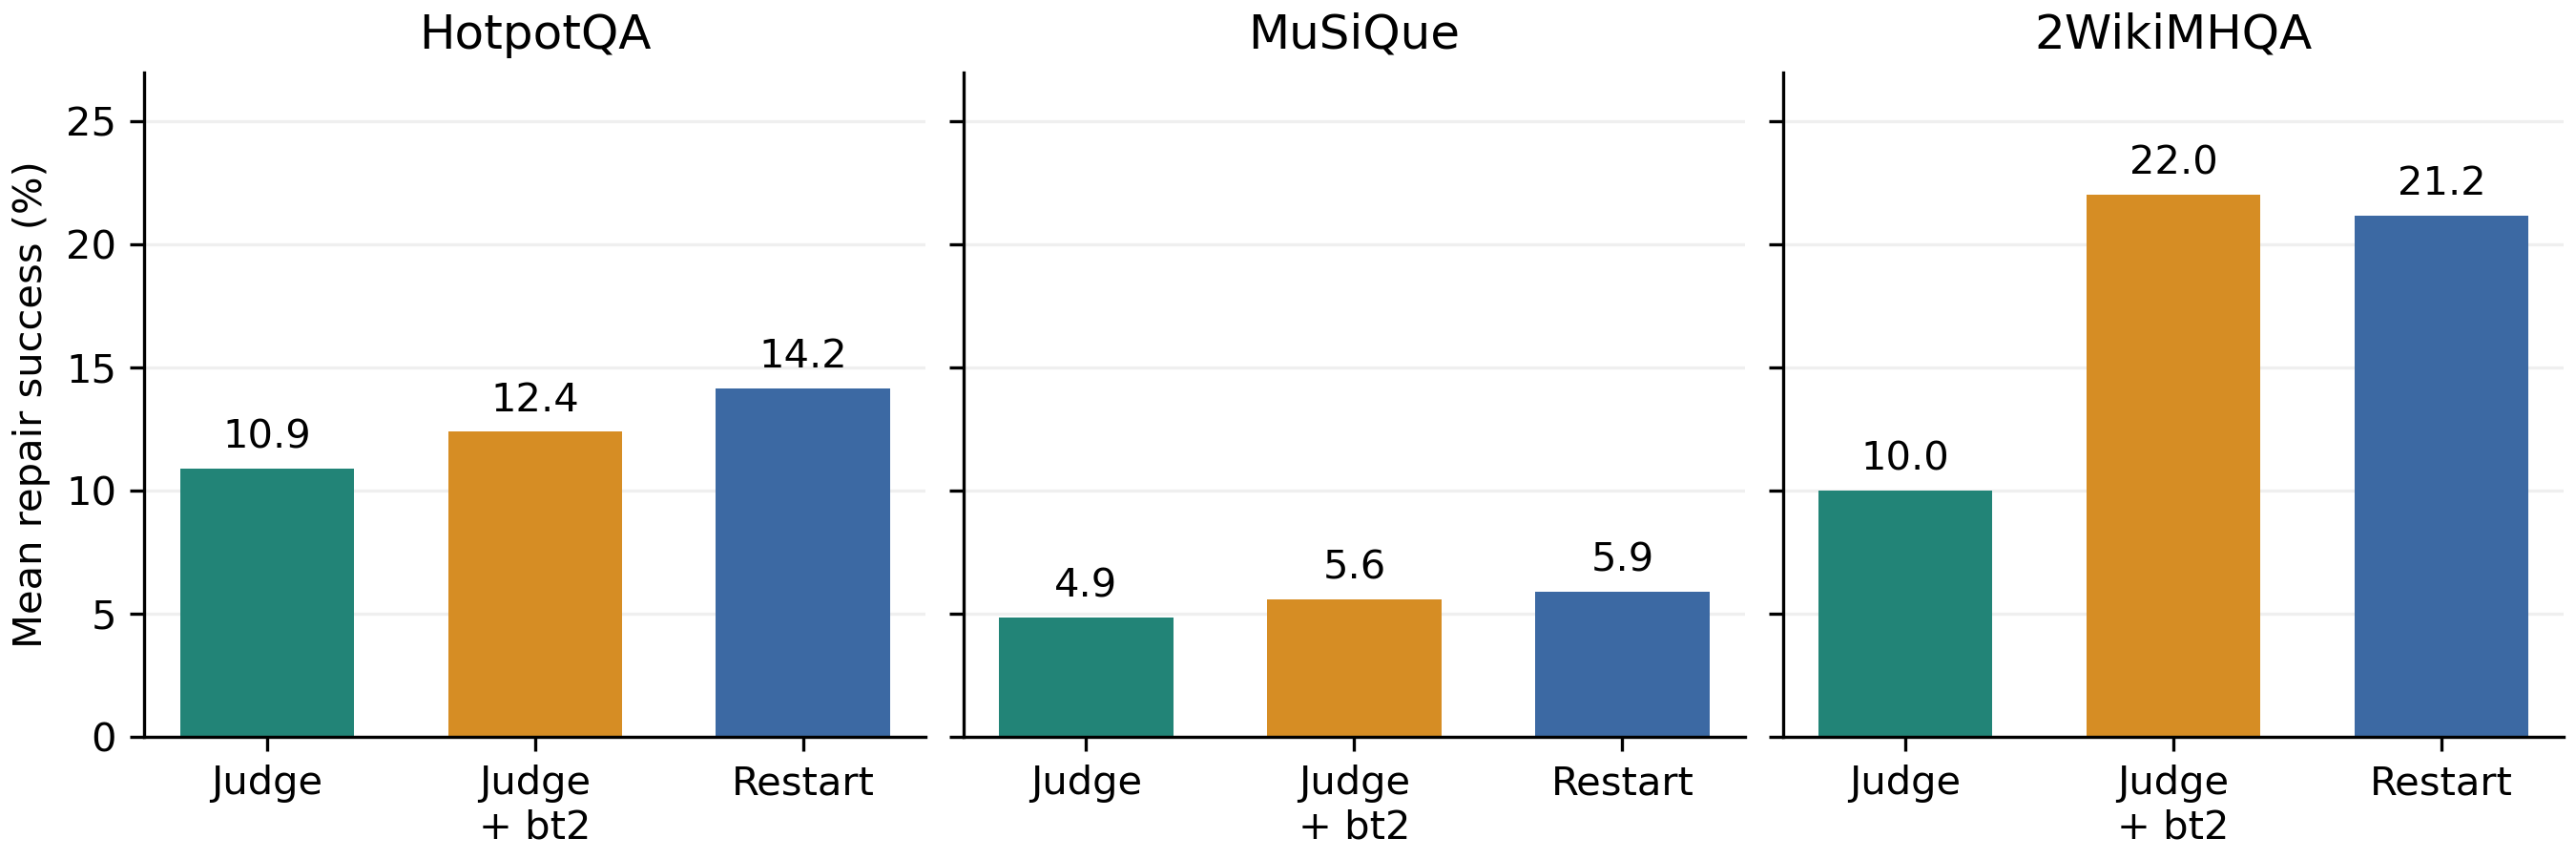
\includegraphics[width=\linewidth]{generated/iclr2027_repair_rates.png}
\caption{Descriptive archived rates for judge-targeted repair, two-step
backtracking, and restart. All bars use mean seed success. The figure
does not encode uncertainty intervals or establish a causal mechanism.}
\label{fig:repair}
\end{figure}

\subsection{RQ2: Moving the Regeneration Origin Upstream}
Backtracking the judge-selected origin increases archived mean success by
\HotpotGain{}, \MusiqueGain{}, and \WikiGain{} percentage points on
HotpotQA, MuSiQue, and 2WikiMultiHopQA. The largest change occurs on
2WikiMultiHopQA: \WikiJudge\% to \WikiBacktrack\%, compared with
\WikiRestart\% for restart. This motivates evaluating earlier recovery
origins. It is not a direct test of error cascades, since backtracking
simultaneously changes retained context, regeneration length, and whether
the judge's selected step remains relevant.

There are two distinct questions within this comparison. An offset can
improve a given localizer by preserving less context; it can also make
many localizers operationally identical by clamping them to zero. The
aggregate gains cannot distinguish these cases. A per-question analysis
should report the selected origin before and after the offset, the fraction
of interventions becoming restarts, and the gain among those retaining a
nonempty prefix. These quantities require the original selection records.

\subsection{Retrospective Uncertainty Selection}
The aggregate maximum over uncertainty configurations is \HotpotBestUnc\%
on HotpotQA, \MusiqueBestUnc\% on MuSiQue, and \WikiBestUnc\% on
2WikiMultiHopQA. The corresponding saved notebook identifies an informed
probability-complement/top-three variant on HotpotQA, an informed
perplexity/position-weighted/backtrack-two variant on MuSiQue, and a
generic perplexity/top-three/backtrack-two variant on 2WikiMultiHopQA.
These are selected on the same questions used to report their success.
Their rates describe the explored grid, not the expected performance of
a policy chosen without looking at test outcomes. In particular, the
first two maxima do not isolate uncertainty from judge-provided hints.

\subsection{RQ3: Localization Is a Separate Outcome}
Action disagreement has the largest exact agreement among the five
reported argmax metrics in each dataset (Figure~\ref{fig:localization};
the numeric table is in Appendix~\ref{app:diagnostics}).
The corresponding values are $0.248$, $0.129$, and $0.404$ for HotpotQA,
MuSiQue, and 2WikiMultiHopQA. This ordering concerns the reference label,
not the success of every metric--rule repair combination. A fair random
localization reference must use the eligible steps of each original
trajectory, and requires the underlying records. Likewise, a comparison
of uncertainty with random repair should match backtracking, hint access,
budget, and question coverage, then evaluate a prespecified strategy.

\begin{figure}[t]
\centering

\includegraphics[width=\linewidth]{generated/iclr2027_localization_heatmap.png}
\caption{Exact agreement with the reference error step for argmax
localization. Larger values indicate annotation agreement, not repair
success or calibrated error probabilities. All entries are archived
fractions; human validation is not available in the snapshot.}
\label{fig:localization}
\end{figure}

The signal with the greatest annotation agreement need not be the cheapest
to acquire: action disagreement requires five additional sampled actions
per measured step, whereas stored-token signals reuse the initial rollout.
Nor does the highest agreement establish the best downstream policy. The
reported repair maximum varies both the signal and the localization rule,
sometimes using privileged hints. Comparing that maximum with an argmax
localization score would change multiple factors at once.

\subsection{RQ4: Recovery Cost and Hint Information}
\label{sec:cost}
\paragraph{Generated-token and tool costs.}
Table~\ref{tab:cost} restores the recorded recovery-only costs for the four
baselines. These are rounded means from the same saved displays as their
success rates. They exclude the reused prefix from generated-token counts
but do not measure prompt processing or all policy overhead. They are
therefore descriptive resource measurements, not an audited comparison
at equal total computation.

\begin{table}[t]
\centering
\caption{Archived mean generated recovery tokens and recovery tool calls.
HP: HotpotQA; MS: MuSiQue; 2W: 2WikiMultiHopQA. Prompt, uncertainty,
diagnosis, and selection costs are not included.}
\label{tab:cost}
\small
\begin{tabular}{@{}lrrrrrr@{}}
\toprule
Strategy & HP tokens & HP tools & MS tokens & MS tools & 2W tokens & 2W tools \\
\midrule
Random origin & 182 & 2.80 & 216 & 3.90 & 170 & 2.36 \\
Judge-targeted & 236 & 3.70 & 320 & 5.82 & 171 & 2.26 \\
Judge + backtrack 2 & 272 & 4.51 & 347 & 6.39 & 234 & 3.68 \\
Full restart & 274 & 4.74 & 348 & 6.62 & 246 & 4.03 \\
\bottomrule
\end{tabular}

\end{table}

On HotpotQA, two-step-backtracked judge repair uses 272 generated tokens
and 4.51 tool calls on average, versus 274 and 4.74 for restart, while
its success rate is lower. On MuSiQue the corresponding token means are
347 and 348. Retaining a prefix does not necessarily yield a substantial
generated-token saving. On 2WikiMultiHopQA, backtracked judge repair has
both a lower displayed token mean (234 versus 246) and a higher displayed
success rate (22.0\% versus 21.2\%) than restart. This is a point-estimate
comparison, not statistically established dominance.

\begin{figure}[t]
\centering
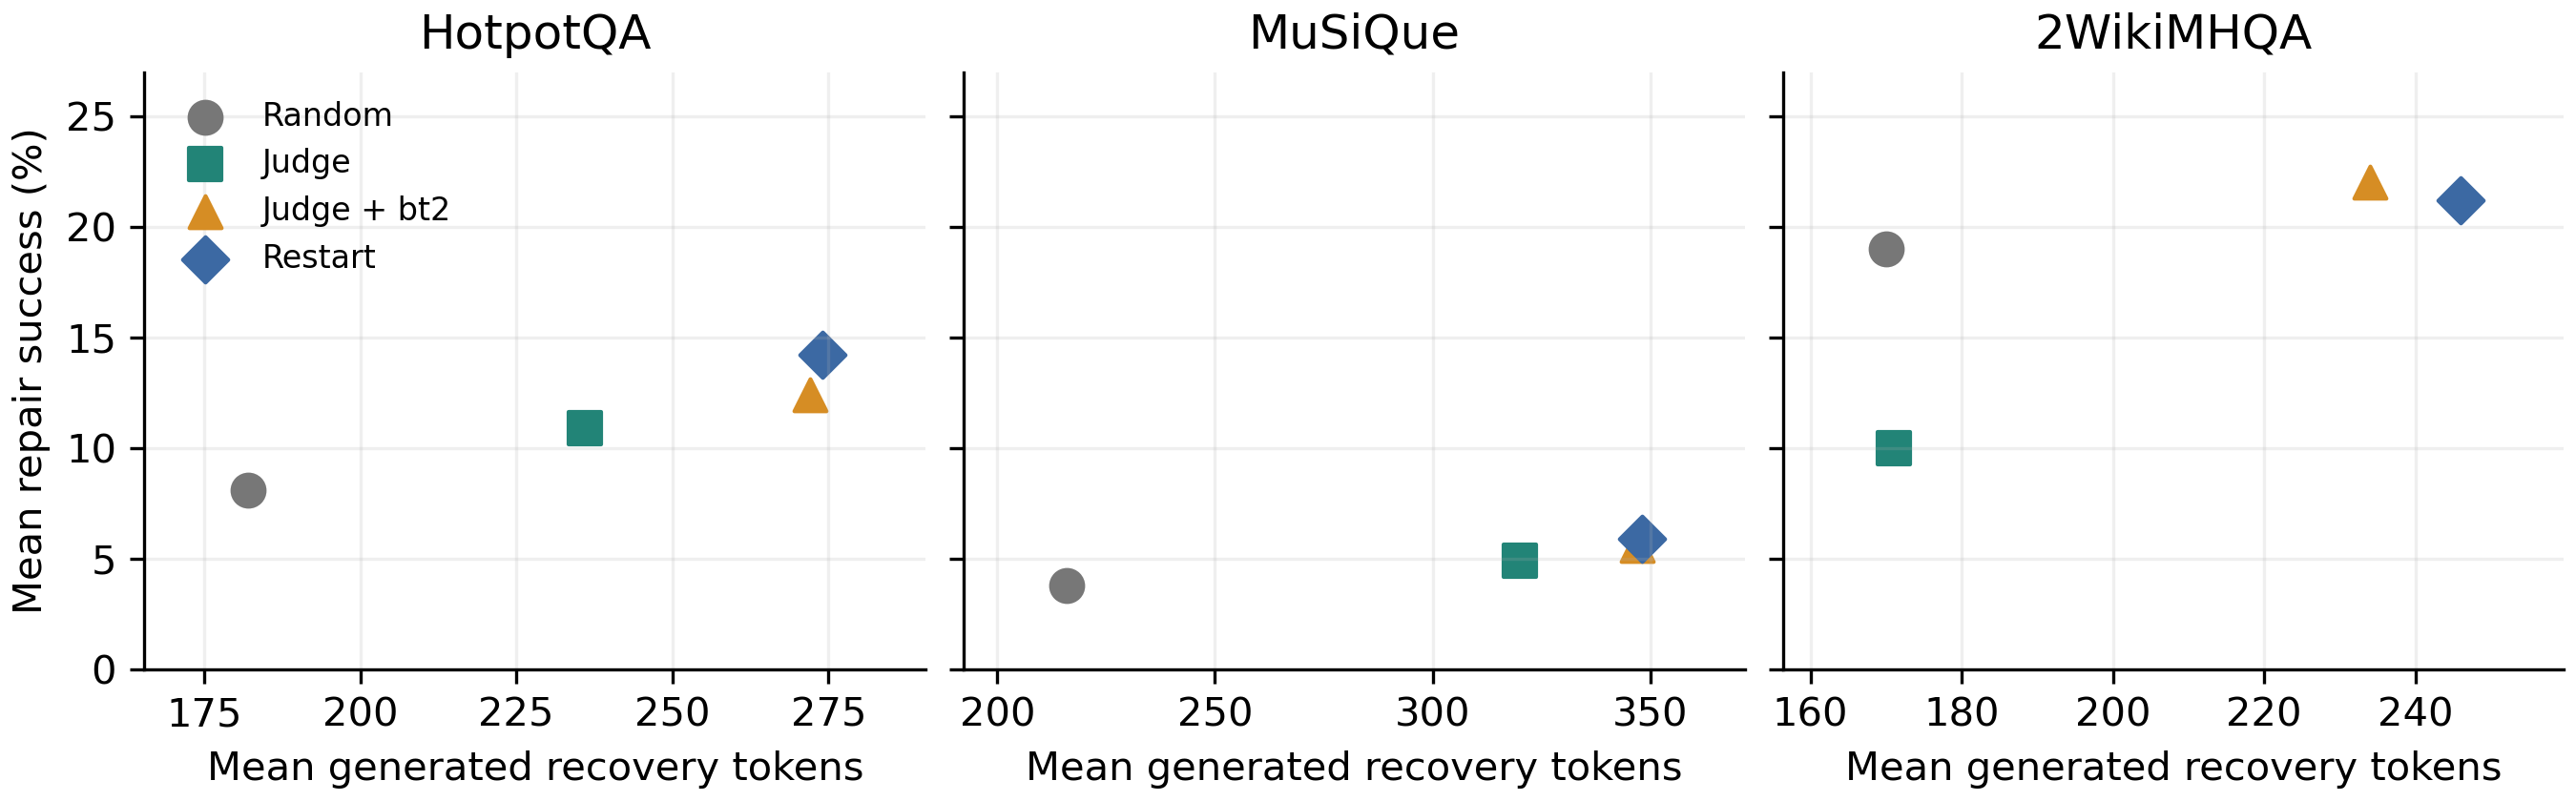
\includegraphics[width=\linewidth]{generated/iclr2027_cost_success.png}
\caption{Recovery-token cost versus success for the four recoverable
baseline summaries. Markers are historical point estimates, with no
confidence intervals. This is not the full-grid Pareto frontier and does
not include all inference costs.}
\label{fig:cost}
\end{figure}

\paragraph{Informed versus generic nudges.}
An origin-preserving hint comparison must keep backtracking fixed.
Table~\ref{tab:nudges} does so for the reference-targeted conditions.
At offset zero, informed hints change the displayed rates by $+0.5$,
$0.0$, and $+2.2$ percentage points; at offset two the changes are $-0.6$,
$0.0$, and $-1.0$. Zero denotes equality at one-decimal display precision,
not exact equality or statistical equivalence. Keeping origins fixed is
necessary to distinguish a hint change from a backtracking change.

\begin{table}[t]
\centering
\caption{Reference-targeted hint comparison at fixed backtrack offsets.
Delta is informed minus generic, in percentage points, calculated from
rounded archived means. Informed hints use the gold-aware annotation.}
\label{tab:nudges}
\small
\begin{tabular}{@{}lrrrr@{}}
\toprule
Dataset & Backtrack & Generic (\%) & Informed (\%) & Delta (pp) \\
\midrule
HotpotQA & 0 & 10.9 & 11.4 & +0.5 \\
HotpotQA & 2 & 12.4 & 11.8 & -0.6 \\
MuSiQue & 0 & 4.9 & 4.9 & +0.0 \\
MuSiQue & 2 & 5.6 & 5.6 & +0.0 \\
2WikiMHQA & 0 & 10.0 & 12.2 & +2.2 \\
2WikiMHQA & 2 & 22.0 & 21.0 & -1.0 \\
\bottomrule
\end{tabular}

\end{table}

The direction varies with the origin, so these summaries support neither
a blanket advantage nor a blanket penalty for more specific hints.
An informed prompt might focus a useful correction, or direct the model
toward an incorrect diagnosis. Distinguishing these explanations requires
paired outcomes and diagnosis-quality annotations. In particular, the
comparison does not demonstrate a gold-free self-correction capability.


\section{Expanded Archived Diagnostics}
\label{app:diagnostics}
\begin{table}[h]
\centering
\caption{Exact reference-step agreement for argmax, underlying
Figure~\ref{fig:localization}. Entries are fractions.}
\label{tab:localization}
\small
\begin{tabular}{@{}lrrr@{}}
\toprule
Metric & HotpotQA & MuSiQue & 2WikiMHQA \\
\midrule
Action disagreement & 0.248 & 0.129 & 0.404 \\
Token entropy (max) & 0.195 & 0.099 & 0.246 \\
Sampled-token complement (max) & 0.177 & 0.099 & 0.232 \\
Perplexity & 0.173 & 0.064 & 0.167 \\
Verbalized uncertainty & 0.088 & 0.085 & 0.059 \\
\bottomrule
\end{tabular}

\end{table}

\begin{figure}[t]
\centering
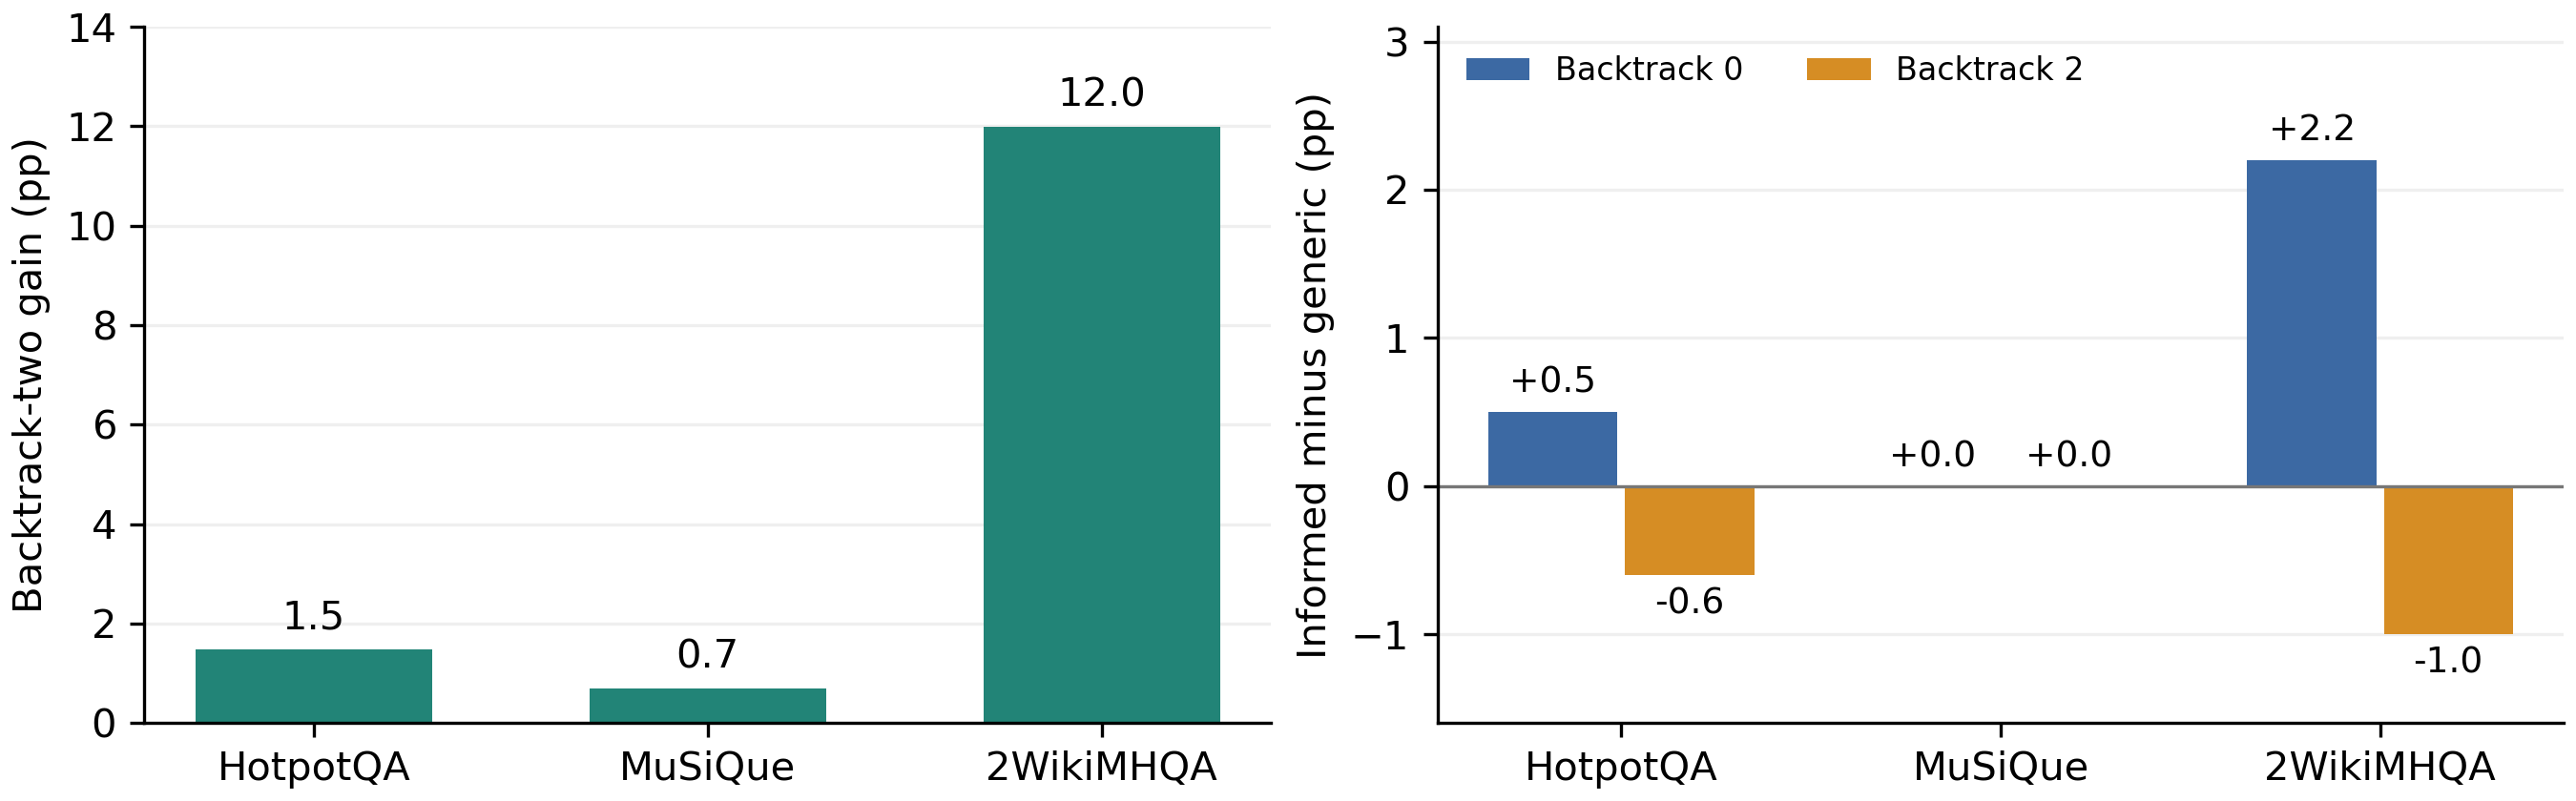
\includegraphics[width=\linewidth]{generated/iclr2027_origin_hint_deltas.png}
\caption{Two descriptive changes in the reference-targeted comparisons.
Left: moving the origin two steps earlier, from archived mean-rate CSVs.
Right: informed minus generic hints at fixed offsets, from rounded saved
notebook displays. Neither panel provides paired confidence intervals.}
\label{fig:deltas}
\end{figure}

\subsection{Candidate Coverage and Recoverable Costs}
The saved ``any uncertainty strategy succeeded'' values are 36.0\% on
HotpotQA, 16.2\% on MuSiQue, and 46.0\% on 2WikiMultiHopQA. The evaluation
code forms this pseudo-strategy by taking the maximum success within each
question and seed over the zero-additional-backtrack uncertainty variants,
including informed variants. It does not select an answer without the
benchmark reference. Also, a rule with zero additional backtracking can
still have an upstream preference built into the localizer.

The associated token totals sum nominal member rows. Because several
members may select the same origin and hint and reuse one generated
suffix, those totals can double-count physical executions. The earlier
47--70-fold compute claim is therefore not retained. These coverage
values describe a candidate set under privileged retrospective selection;
they should not be placed on an operational Pareto frontier alongside
single-output policies. A valid ensemble comparison must freeze a gold-free
selector and count unique candidates, acquisition calls, and selection.

\subsection{Why Seed Aggregation Changes the Question}
For three repair seeds, a question with outcomes $(1,0,0)$ contributes
$1/3$ to the mean one-attempt repair rate and zero to majority repeatability.
A question with $(1,1,0)$ contributes $2/3$ and one, respectively. Both
summaries can be useful, but mixing them across rows changes the estimand.
The restored main table consistently uses mean-success summaries. The
earlier notebook's confidence intervals are not reused because its
row-wise bootstrap does not preserve the question-level dependence.

The available displays show only ten strategy rows out of 127, including
the coverage pseudo-strategy. The reconstruction parses those visible
rows, rejects missing or duplicated required baselines, and checks three
baseline rates against the cross-dataset CSVs. It does not infer the
hidden rows, reconstruct their joint outcome distribution, or treat rounded
costs as exact measurements. This distinction is why the cost plot shows
baseline points rather than recreating a full-grid Pareto boundary.

\subsection{Legacy Interpretation Limits}
\paragraph{Context effects are hypotheses.}
The possibility that retained errors constrain recovery is consistent
with the observed benefit of changing origins. However, the archived
``trajectory length'' statistic is the average number of tool calls in
full-restart repairs. It is a post-intervention outcome, not the original
failed trajectory's length. Correlating four dataset averages cannot
justify a four-step routing threshold. Testing the role of prefix context
requires original lengths, within-dataset comparisons, and interventions
that manipulate the prefix while holding other factors constant.

\paragraph{Error propagation versus recovery opportunity.}
Backing up a rollout removes later reasoning and observations, but under
the historical total-step limit it also grants more new agent turns.
Both changes can improve repair without proving that the first retained
error caused a downstream uncertainty peak. An error-cascade explanation
requires showing the ordering of reference errors and uncertainty peaks,
then testing whether the proposed upstream intervention improves recovery
beyond a position-matched control. A controlled new-step regime separates
some of these factors; the historical total-step regime remains a useful,
separately labeled operational setting.

\paragraph{Failure-mode analysis.}
Two hypotheses are an error preceding the uncertainty peak and legitimate
uncertain exploration. The first requires the proportion of localization
misses with $k_J<k_U$, its denominator, and annotation source. The existing
exploration flag only identifies missed \texttt{search}/\texttt{lookup}
actions, not their correctness. These overlapping hypotheses do not
establish the originally asserted 70\% and 20\% prevalences.

\paragraph{Candidate coverage is not answer selection.}
An ``any strategy succeeded'' aggregate uses benchmark answers, so it
measures retrospective coverage, not operational ensemble accuracy.
Deployment requires a gold-free selector and costs for unique executions
and selection; summing nominal strategy costs double-counts shared work.

\paragraph{From diagnosis to a repair policy.}
A policy must select an origin before observing its repair outcome.
Predicting judge agreement does not establish repair utility, and selecting
the best test rollout is retrospective. The completed study evaluates six
prespecified conditions with matched hints and allowances. An all-origin
matrix is deferred; neither an origin-wide optimum nor an all-origin cost
frontier is estimated. Appendix~\ref{app:completion} separates completed work
from deferred extensions.

The practical implication concerns evaluation: measure recovery directly,
include restart, and separate information access from origin selection.
The results justify neither a length router, an advantage over
diagnosis-and-replay, nor deployment of a gold-selected ensemble.

\section{Completed Controlled Protocol, Audit and Costs}
\label{app:completion}
This appendix records the completed HotpotQA experiment. The protocol and
cohort were frozen before new outcomes, but were not publicly preregistered.
Historical results elsewhere in the paper are not relabeled as its outcomes.

\subsection{Frozen Conditions and Model}
The main model and tokenizer snapshot was
\texttt{Qwen/Qwen2.5-32B-Instruct-AWQ}, revision
\path{5c7cb76a268fc6cfbb9c4777eb24ba6e27f9ee6c}. The run used one AWS
London \texttt{g7e.2xlarge} with a 96GB RTX PRO 6000 GPU. Initial generation
was greedy; repairs used temperature $0.7$, seeds $0,1,2$ and batch size two.
Every repair had at most eight new steps, 512 generated tokens per step,
and total cap $B_q=G_q$, the original failed trajectory's generated-token
count. The complete failed trace's uncertainty profile selects the origin;
the recovery prompt contains only the retained prefix and generic hint.
The discarded suffix and reference labels are not inserted into that prompt.

\begin{table}[h]
\centering
\caption{The six frozen conditions actually evaluated. $k_U$ is the
perplexity argmax, $J$ a uniform draw over eligible original steps, and
$K_{\mathrm{dev}}$ the mapped development-profile draw described below.
Every condition has the same hint and recovery allowance.}
\label{tab:budget_protocol}
\small
\begin{tabular}{@{}ll@{}}
\toprule
Condition & Effective origin \\
\midrule
Full restart & $0$ \\
Offset-matched random & $\max(0,J-2)$, $J\sim\operatorname{Unif}\{0,\ldots,T-1\}$ \\
Fixed early (descriptive) & $\min(1,T-1)$ \\
Uncertainty + backtrack 2 & $\max(0,k_U-2)$ \\
Position-matched random & $K_{\mathrm{dev}}$ \\
Uncertainty, no backtrack & $k_U$ \\
\bottomrule
\end{tabular}
\end{table}

The position profile contains 24 failed original development trajectories;
its effective-origin counts are 14 at zero, two at one, five at three, one
at four and two at five. It uses no development repair outcomes. For a
uniformly sampled development entry $j$ with origin $k_j$ and length $T_j$,
the new origin is
\begin{equation}
 K_{\mathrm{dev}}=\left\lfloor
 \frac{k_j}{\max(1,T_j-1)}(T_q-1)+\frac12\right\rfloor.
\end{equation}
The profile and seeded sampling were frozen before test outcomes. This is
a normalized-position mapping, not a fitted conditional model for every
possible trajectory length. All 50 development source questions are excluded.
The six conditions and three seeds allow at most $18N$ unique repair jobs
for $N$ failures; shared effective executions reduced 2,034 rows to 1,058 jobs.

\subsection{Cohort Reconstruction and Immutable Evidence}
The historical 500-question pool was reconstructed with the original
sampler at git commit \texttt{7a73907}, seed 42, stratification by level and
type, and the archived 7,405-record dataset. Its union with 60 AWS development
IDs contains 549 distinct exclusions. The original pool file's displayed
date, size and one visible question ID corroborate the reconstruction;
they are not a comparison of its full contents. Undocumented historical
runs cannot be excluded. The remaining 6,856 sorted IDs supplied the
250-question cohort, sampled without replacement using seed 20260912.

The freeze was recorded on September 12 at 03:27:45 UTC, before the
04:06:56 EC2 start request and 04:11:45 batch-runner start. The five batches
were completed and pooled at 05:25:03 UTC without outcome-based changes.
The immutable identities are:
\begin{itemize}
\item Study:\\
{\footnotesize\path{e4ea08c8291b0f797d05b15110d762634ec48d57ae53e05aaf4373c805986308}}.
\item Source:\\
{\footnotesize\path{b418bca20be1674d65dc76dc14c42f2b6304eee6856d34a6f083c3d4e6ef4eb9}}.
\item Raw dataset:\\
{\footnotesize\path{a9b4c5906587ac0d20eb83dcb29d0240e268e342c170f7f22988f59f13fa82c3}}.
\item Position profile:\\
{\footnotesize\path{3e4e834cca3857f409d0dae0baf710658825687883bc1ae5eeaf1ebb9c02bb8c}}.
\end{itemize}
The local reproducibility record includes \texttt{study-freeze.json},
\texttt{test-ids-250.json}, \texttt{historical-reconstruction.json},
\texttt{archive-verification.json} and all five executed batch archives.
The source identity above is distinct from the individual ZIP/archive checksums.

\subsection{Question-Level Inference and Secondary Outcomes}
All five batches are pooled with equal question weight after averaging
seeds. Individual 95\% intervals use 10,000 paired question bootstrap
resamples with analysis seed zero. The sign-flip tests assume
within-question exchangeability; four primary $p$-values receive one Holm
correction. Fixed early remains descriptive. The intervals themselves
are not simultaneous family-wise intervals.

\begin{table}[h]
\centering
\caption{Prespecified treatment-minus-control comparisons in repair success,
in percentage points. All use 113 paired question means. Intervals are
individual 95\% bootstrap intervals; $p$-values are paired sign-flip tests.}
\label{tab:main_contrasts}
\small
\begin{tabular}{@{}lrrrr@{}}
\toprule
Control & Delta (pp) & 95\% interval (pp) & Raw $p$ & Holm $p$ \\
\midrule
Full restart & -1.47 & [-4.13, +0.88] & 0.358 & 1.000 \\
Random + backtrack 2 & -0.88 & [-4.13, +2.06] & 0.695 & 1.000 \\
Position-matched random & +0.00 & [-2.95, +2.95] & 1.000 & 1.000 \\
Uncertainty, no backtrack & +1.18 & [-2.95, +5.31] & 0.682 & 1.000 \\
\bottomrule
\end{tabular}

\end{table}

Strict exact match and continuous answer F1 are exploratory sensitivities
on the same 113 failures. Their full paired outputs are preserved in
\texttt{pooled-analysis-local.json}; they are not substituted for the
primary gate or its comparison family. Changing to an EM-only failure
gate would include additional initially accepted questions for which this
experiment did not run repairs. Three seeds per question do not triple
the sample size. An ideal reference-gated overall success rate would be
$A_0+(1-A_0)R_a$ when initially successful answers are left untouched;
this identity does not measure a deployed detector's false alarms or regressions.

\subsection{Independent Artifact Audit}
All 180 CPU tests and all 22 plan-only notebook cells passed before launch.
Each completed batch was archived with a checksum and independently checked
after retrieval. The auditor loaded the frozen source bundle, verified
source/input hashes, reconstructed prespecified origins and prompts,
checked full question/seed/condition coverage, replayed tool observations,
and recomputed answer metrics with the official HotpotQA reference scorer.

\begin{table}[h]
\centering
\caption{Completed batch coverage. Violations include replay/scoring
mismatches and generated-token/new-step allowance violations; every count is zero.}
\label{tab:main_audit}
\small
\begin{tabular}{@{}lrrrrr@{}}
\toprule
Batch & Initial & Failed & Unique repairs & Condition/seed rows & Violations \\
\midrule
1 & 50 & 20 & 195 & 360 & 0 \\
2 & 50 & 21 & 212 & 378 & 0 \\
3 & 50 & 25 & 223 & 450 & 0 \\
4 & 50 & 21 & 196 & 378 & 0 \\
5 & 50 & 26 & 232 & 468 & 0 \\
\bottomrule
\end{tabular}

\end{table}

The audit covers \MainTrajectories{} trajectories, \MainObservations{}
observations, \MainPrefixes{} retained prefix steps, 241 input hashes and
2,034 origin/prompt checks. It found zero mismatches and zero token or
new-step violations. Local pooling of the retrieved records agrees with
the AWS analysis within $10^{-12}$. These checks verify the saved evidence
and local tool replay, not bitwise reproduction of stochastic continuations
or independent human validation of reference judgments.

\subsection{Infrastructure Usage and Cost Limits}
The run had a US\$25 gross allowance inside the original US\$119 allocation.
Guest powerdown was recorded at 05:28:11 UTC. After a retrieval-only restart
at 08:48:58, AWS recorded a user-initiated stop reason at 08:54:09 and was
observed stopping at 08:55:59. The instance was independently confirmed
stopped with no public IP at 19:02:37. No inference was repeated for retrieval.

The cost worksheet uses the verified US\$5.84531/hour rate, approximately
81.25 minutes through main guest powerdown, and a conservative 7.01-minute
retrieval interval through the observed stopping state. It adds a one-minute
main-transition contingency, retained 200 GiB gp3 storage, and a conservative
IPv4 allowance through September 12 at 19:03:19 UTC. The exact provider
transition time after main guest powerdown was not captured; the one-minute
contingency is an assumption, not a verified upper bound.

\begin{table}[h]
\centering
\caption{Estimated infrastructure usage through the recorded report cutoff.
This is not an AWS invoice or a matched-total-compute comparison.}
\label{tab:main_cost}
\small
\begin{tabular}{@{}lr@{}}
\toprule
Component & Estimated USD \\
\midrule
Main compute through guest powerdown & 7.915 \\
Retrieval through observed stopping & 0.683 \\
One-minute transition contingency & 0.097 \\
Retained storage through report cutoff & 0.385 \\
Conservative public IPv4 allowance & 0.075 \\
Total before credits, tax and transfer & 9.16 \\
\bottomrule
\end{tabular}

\end{table}

The estimate is US\$\MainEstimatedUSD{} before credits, tax and transfer;
unrelated account workloads and later storage are excluded. Retained storage
continues at approximately US\$0.62/day. Original generation used 57,499
generated tokens and unique repairs used 303,700 generated and 5,292,100
prompt tokens. Acquisition, prefix processing, tool latency, batching and
selection must be accounted for to support a policy-efficiency claim;
these totals alone do not supply that comparison.

\subsection{Separate Follow-up and Deferred Scientific Work}
The six-condition study does not include a diagnosis/replay comparator or
additional token allowances. These comparisons were subsequently completed
on a separate cohort (Section~\ref{sec:diagnosis_followup}). Replication on
the other two QA datasets, a second model, matched runtime, a full-origin
matrix and new 72B reference annotations are outside these completed studies. FEVER
remains excluded because its inspected loader substituted claim text for
retrieved evidence. MuSiQue conversion and answer-alias handling require
their own provenance/scoring audit before a corrected run.

Historical localization claims still require independent human judgments.
The existing proposal samples 50 failed traces per QA dataset independently
of repair success, with two annotators blinded to judge labels and outcomes:
150 trajectories and 300 initial judgments. Individual judgments and
adjudication would be preserved separately, with ambiguity and multiple-error
cases allowed. No such annotations or annotator labor were supplied here.
Context interventions and original-length analyses would require separately
declared hypotheses; this paper does not infer error-cascade prevalence or
a trajectory-length routing threshold from the archived averages.

\section{Review-Stage Diagnostics}
\label{app:review_diagnostics}
These exploratory analyses were added after the primary study completed.
They retain all 250 initial questions, 113 failures, six conditions and three
seeds. The diagnostic loader verifies 398 input-to-archive comparisons against
the five checksummed archives, rescoring original and repaired answers and
rejecting missing trials, inconsistent shared executions or allowance
violations. Exported trial and initial-question CSVs, the analysis-code
hashes and the review-stage analysis plan accompany the diagnostic JSON.
The original primary estimates and Holm family are unchanged.

\subsection{Policy Costs and Termination}
Costs in Table~\ref{tab:review_costs} average seeds within each question.
Each standalone policy pays for the execution it would use, even if that
execution was shared with another condition during this experiment. The
study's infrastructure totals instead deduplicate physical executions.
All six policies use stored information and incur zero additional
selection-model requests. CPU scoring, log-probability extraction, cache
behavior and scheduling overhead are not measured by token totals.

\begin{table}[h]
\centering\footnotesize
\caption{Exploratory mean recovery usage per attempted repair, on 113
questions and three seeds. F/B/S are counts terminating with an answer,
at the token budget, or at the new-step limit; each row sums to 339.
Prompt and output tokens are separate quantities, not an estimate of FLOPs.}
\label{tab:review_costs}
\begin{tabular}{@{}lrrrrr@{}}
\toprule
Condition & Output tokens & Prompt tokens & Requests & Tool calls & F / B / S \\
\midrule
Full restart & 271.6 & 3153.3 & 5.26 & 4.54 & 162 / 99 / 78 \\
Random + backtrack 2 & 268.4 & 4179.6 & 5.15 & 4.40 & 171 / 97 / 71 \\
Fixed early (descriptive) & 258.1 & 3720.6 & 4.82 & 4.07 & 193 / 75 / 71 \\
Uncertainty + backtrack 2 & 269.9 & 4083.3 & 5.11 & 4.35 & 171 / 103 / 65 \\
Position-matched random & 264.5 & 3885.8 & 5.01 & 4.26 & 178 / 90 / 71 \\
Uncertainty, no backtrack & 255.6 & 5077.3 & 4.77 & 3.99 & 186 / 91 / 62 \\
\bottomrule
\end{tabular}

\end{table}

A repair can reach its token cap on a request that also emits a final
answer or reaches the step limit. Consequently, the recorded termination
reason and token-cap equality are different diagnostics: treatment has
103 budget-labelled stops but 152/339 executions use their complete token
cap. There is no zero-token allowance in this study. Initial failures
comprise 61 completed incorrect answers and 52 original step-limit stops.
A different allowance requires separate executions; it cannot
be reconstructed by reweighting these stopped traces.

\subsection{Secondary Metrics and the Actual Failure Gate}
\begin{table}[h]
\centering\footnotesize
\caption{Exploratory treatment-minus-control differences on the same 113
initial failures. Individual 95\% question-bootstrap intervals are not
adjusted for the eight secondary comparisons. EM is in percentage points;
F1 differences are multiplied by 100. The original primary tests use the
answer-success gate, not these metrics.}
\label{tab:review_sensitivity}
\begin{tabular}{@{}lrr@{}}
\toprule
Control & EM delta [95\% CI], pp & 100$\Delta$F1 [95\% CI] \\
\midrule
Full restart & -1.47 [-3.83, +0.59] & -1.67 [-4.28, +0.64] \\
Random + backtrack 2 & +0.29 [-2.06, +2.65] & -1.27 [-4.14, +1.45] \\
Position-matched random & +1.47 [-0.59, +3.83] & +0.11 [-2.48, +2.62] \\
Uncertainty, no backtrack & +2.95 [+0.29, +5.60] & +1.80 [-1.35, +5.07] \\
\bottomrule
\end{tabular}

\end{table}

\begin{table}[h]
\centering\small
\caption{Outcomes over all 250 questions under the implemented reference
gate: preserve initially accepted answers and apply one sampled repair only
to the original 113 failures. Three seeds estimate that repair's mean
outcome. Initial rates were 54.80\% gate success, 38.80\% EM and 0.5164 F1.
These are not outcomes of an EM-only rerun or a deployed failure detector.}
\label{tab:review_population}
\begin{tabular}{@{}lrrr@{}}
\toprule
Recovery condition & Gate success (\%) & EM (\%) & F1 \\
\midrule
Full restart & 59.87 & 42.67 & 0.5597 \\
Random + backtrack 2 & 59.60 & 41.87 & 0.5579 \\
Fixed early (descriptive) & 60.00 & 41.20 & 0.5564 \\
Uncertainty + backtrack 2 & 59.20 & 42.00 & 0.5522 \\
Position-matched random & 59.20 & 41.33 & 0.5517 \\
Uncertainty, no backtrack & 58.67 & 40.67 & 0.5440 \\
\bottomrule
\end{tabular}

\end{table}

The full-cohort calculation retains the same 40 F1-accepted but non-EM
original answers for every policy. It never treats the reference gate as a
learned detector and never uses majority-over-seeds voting or an oracle
best-of-three selector. Question-bootstrap intervals for these descriptive
rates are included in the diagnostic JSON.

\subsection{Illustrative Traces and Selection Rule}
For each of three outcome strata---higher treatment seed mean, higher restart
seed mean, or zero success for both---we display the first sorted question ID
and all three seeds. These outcome-selected cases illustrate measured behavior;
they do not estimate prevalence, validate diagnoses or establish corrected
causal mechanisms. F1 uses each full displayed answer; none of the 18 answers
passes strict EM.

\par\medskip\noindent\begin{minipage}{\linewidth}
\paragraph{Case 1: Higher treatment seed mean.}
\textit{In 1632, where was one of the most highly acclaimed English architects born?} Reference answer: East Knoyle. The original trace has 8 steps and a 439-token recovery allowance.
\begin{center}\footnotesize
\begin{tabular}{@{}p{.20\linewidth}rp{.16\linewidth}p{.44\linewidth}@{}}
\toprule Condition & Origin & Gate; F1, seeds 0/1/2 & Answers, seeds 0/1/2 \\
\midrule
Restart & 0 & 0/0/0; 0.00/0.00/0.00 & \textit{no answer}; \textit{no answer}; \textit{no answer} \\
Uncertainty + bt2 & 3 & 0/0/1; 0.00/0.00/0.67 & \textit{no answer}; \textit{no answer}; East Knoyle, Wiltshire, England \\
\bottomrule\end{tabular}\end{center}
Question ID: \texttt{5a7619765542992db9473728}.
\end{minipage}\par
\par\medskip\noindent\begin{minipage}{\linewidth}
\paragraph{Case 2: Higher restart seed mean.}
\textit{Was the Metropolitan Life Insurance Company Tower [Met Life Tower] or the 15 Hudson Yards building designed by the firm of Napoleon LeBrun \& Sons?} Reference answer: The Metropolitan Life Insurance Company Tower. The original trace has 8 steps and a 458-token recovery allowance.
\begin{center}\footnotesize
\begin{tabular}{@{}p{.20\linewidth}rp{.16\linewidth}p{.44\linewidth}@{}}
\toprule Condition & Origin & Gate; F1, seeds 0/1/2 & Answers, seeds 0/1/2 \\
\midrule
Restart & 0 & 0/0/1; 0.31/0.32/0.62 & The Metropolitan Life Insurance Company Tower was designed by Napoleon LeBrun \& Sons, but there is no information to suggest that 15 Hudson Yards was designed by the same firm.; The Metropolitan Life Insurance Company Tower was designed by Napoleon LeBrun \& Sons, but there is no information to suggest that 15 Hudson Yards was designed by them.; The Metropolitan Life Insurance Company Tower was designed by Napoleon LeBrun \& Sons. \\
Uncertainty + bt2 & 4 & 0/0/0; 0.31/0.00/0.15 & The Metropolitan Life Insurance Company Tower was designed by Napoleon LeBrun \& Sons, but there is no information to suggest that Napoleon LeBrun \& Sons designed the 15 Hudson Yards building.; \textit{no answer}; The Met Life Tower was designed by Napoleon LeBrun \& Sons, but the design firm for 15 Hudson Yards is not mentioned in the provided information. \\
\bottomrule\end{tabular}\end{center}
Question ID: \texttt{5a7322a25542991f9a20c634}.
\end{minipage}\par
\par\medskip\noindent\begin{minipage}{\linewidth}
\paragraph{Case 3: Both policies unsuccessful.}
\textit{Which movie is loosley based off the Brother Grimm's "Iron Henry"?} Reference answer: The Frog Prince. The original trace has 8 steps and a 382-token recovery allowance.
\begin{center}\footnotesize
\begin{tabular}{@{}p{.20\linewidth}rp{.16\linewidth}p{.44\linewidth}@{}}
\toprule Condition & Origin & Gate; F1, seeds 0/1/2 & Answers, seeds 0/1/2 \\
\midrule
Restart & 0 & 0/0/0; 0.00/0.00/0.00 & \textit{no answer}; \textit{no answer}; \textit{no answer} \\
Uncertainty + bt2 & 5 & 0/0/0; 0.00/0.00/0.00 & There is no; \textit{no answer}; \textit{no answer} \\
\bottomrule\end{tabular}\end{center}
Question ID: \texttt{5a733b835542991f9a20c6b2}.
\end{minipage}\par


\subsection{Precision and Further Evidence}
The 43-question nonzero-origin comparison has a 95\% interval
[$-10.85,+2.33$] percentage points. Its width limits any claim about targeted
repair when a prefix is actually retained. For prospective planning,
$n\simeq1.96^2\widehat\sigma_d^2/h^2$ estimates the independent questions
needed for an individual 95\% interval half-width $h$, using the observed
variance of paired question differences. For a two-point half-width, the
four comparisons give approximately 179, 257, 248 and 476 failed questions,
in the order of Table~\ref{tab:main_contrasts}. These are design sensitivities,
not observed power, guaranteed future precision, simultaneous intervals or
an outcome-dependent stopping rule for the completed study.

Each additional experiment must declare its scope and affordable sample
size before new outcomes. The separate follow-up now evaluates a same-model
diagnosis/replay adaptation and three recovery-token allowances
(Section~\ref{sec:diagnosis_followup}). Independently generated second-model
cohorts would test transportability, while measured complete-policy latency
would address resource questions beyond matched recovery-token caps.
Human labels are required for new error-localization or mechanism claims,
but are not substituted for the deterministic answer scorer in the present
primary comparison.

\section{Diagnosis Follow-up: Complete Results and Costs}\label{app:diagnosis_followup}
The follow-up freezes five batches of 50 new HotpotQA questions before
outcomes. Its 250 IDs exclude the 799 documented earlier IDs. Initial
generation succeeds on 132 questions (52.8\%); 89 are exact matches
(35.6\%) and mean answer F1 is 0.4980. Each of the 118 failures receives
three policies, three seeds, and three allowances, for 3,186 logical rows.
The Qwen32B revision, common retry hint, and eight-new-step allowance match
the earlier study. Generation uses temperature zero; repairs use 0.7.

\begin{table}[ht]
\centering\small
\caption{Separate diagnosis follow-up. Each policy/allowance has 354 seed
trials on the same 118 initial failures. Success is answer EM or F1 at least
0.5. EM and F1 retain that failure cohort.}
\label{tab:diagnosis_results}
\begin{tabular}{@{}lrrrrr@{}}
\toprule
Allowance & Policy & Successes & Success (\%) & EM (\%) & F1 \\
\midrule
$0.5\times$ & Restart & 10/354 & 2.82 & 2.54 & 0.0303 \\
$0.5\times$ & Uncertainty, backtrack 2 & 10/354 & 2.82 & 2.54 & 0.0286 \\
$0.5\times$ & Diagnosis/replay & 15/354 & 4.24 & 3.67 & 0.0649 \\
$1\times$ & Restart & 37/354 & 10.45 & 7.63 & 0.1206 \\
$1\times$ & Uncertainty, backtrack 2 & 35/354 & 9.89 & 7.06 & 0.1122 \\
$1\times$ & Diagnosis/replay & 36/354 & 10.17 & 7.91 & 0.1306 \\
$2\times$ & Restart & 44/354 & 12.43 & 9.32 & 0.1654 \\
$2\times$ & Uncertainty, backtrack 2 & 39/354 & 11.02 & 8.19 & 0.1500 \\
$2\times$ & Diagnosis/replay & 39/354 & 11.02 & 9.32 & 0.1515 \\
\bottomrule
\end{tabular}

\end{table}

\begin{table}[ht]
\centering\small
\caption{Uncertainty minus control in the diagnosis follow-up. Intervals
are individual, unadjusted 95\% question-bootstrap intervals (10,000
resamples). All six two-sided question sign-flip tests share one Holm family.}
\label{tab:diagnosis_contrasts}
\begin{tabular}{@{}lrrrrr@{}}
\toprule
Allowance & Control & $\Delta$ (pp) & 95\% interval (pp) & $p$ & $p_{\rm Holm}$ \\
\midrule
$0.5\times$ & Restart & +0.00 & [-2.26, +2.26] & 1.000 & 1.000 \\
$0.5\times$ & Diagnosis/replay & -1.41 & [-4.52, +1.41] & 0.471 & 1.000 \\
$1\times$ & Restart & -0.56 & [-3.67, +2.54] & 0.876 & 1.000 \\
$1\times$ & Diagnosis/replay & -0.28 & [-4.24, +3.39] & 1.000 & 1.000 \\
$2\times$ & Restart & -1.41 & [-4.80, +1.41] & 0.492 & 1.000 \\
$2\times$ & Diagnosis/replay & +0.00 & [-3.67, +3.39] & 1.000 & 1.000 \\
\bottomrule
\end{tabular}

\end{table}

Diagnosis uses the same model with temperature zero, a 512-token maximum,
and one deterministic seed. The response supplies an integer origin and
a reason. Only the origin controls repair; neither its prose nor discarded
suffix evidence is added to the retry prompt. A malformed response would
fall back to restart and retain its cost; none of the 118 diagnoses required
that fallback. Reference labels determine failure eligibility but do not
enter diagnosis or recovery prompts. This is an untrained origin-selection
adaptation, not a trained-method reproduction.

\begin{table}[ht]
\centering\small
\caption{Mean incremental resource use per standalone recovery attempt,
including a complete diagnosis charge for diagnosis/replay. Generated-token
allowances apply to recovery; prompt processing and diagnosis add cost.}
\label{tab:diagnosis_costs}
\begin{tabular}{@{}lrrrr@{}}
\toprule
Allowance & Policy & Generated & Prompt & Requests \\
\midrule
$0.5\times$ & Restart & 151.3 & 1463.2 & 3.49 \\
$0.5\times$ & Uncertainty, backtrack 2 & 151.6 & 2146.9 & 3.41 \\
$0.5\times$ & Diagnosis/replay & 188.5 & 3289.1 & 4.19 \\
$1\times$ & Restart & 274.3 & 3311.8 & 5.38 \\
$1\times$ & Uncertainty, backtrack 2 & 274.6 & 4504.8 & 5.36 \\
$1\times$ & Diagnosis/replay & 296.1 & 5371.0 & 5.84 \\
$2\times$ & Restart & 295.5 & 3522.6 & 5.56 \\
$2\times$ & Uncertainty, backtrack 2 & 295.1 & 4710.7 & 5.53 \\
$2\times$ & Diagnosis/replay & 311.3 & 5555.6 & 5.97 \\
\bottomrule
\end{tabular}

\end{table}

Physical execution sharing yields 2,079 unique repairs and 118 diagnoses.
Independent audits replay and rescore 2,329 original/repair trajectories,
check 13,504 observations, 2,637 retained prefix steps, and 388 input hashes,
and find zero mismatches. Unique repairs use 496,780 generated tokens,
7,763,726 prompt tokens, and 9,731 model requests; diagnoses use 4,756
generated tokens, 145,641 prompt tokens, and 118 requests. A finish action
counts as a model request, not a retrieval call. The pooled local analysis
matches all 3,186 remote trial rows and 455 numeric results within $10^{-12}$.

An earlier development audit erroneously counted finish as retrieval; it
stopped before any main question. The corrected auditor and a failing-first
regression test changed neither the cohort nor its model, prompts, seeds,
allowances, or planned comparisons. Failed attempts remain preserved.
The conservative infrastructure estimate for all diagnosis attempts and
retrievals is \$18.29, excluding tax and transfer. The completed records
support token and request accounting, not equal runtime or FLOPs.

\section{Related-Work Comparison and Required Controls}
\label{app:related}
This focused literature update uses primary sources available on
September 9, 2026; it is not an exhaustive survey. Table~\ref{tab:related}
compares designs, not repair rates across incompatible cohorts.

\begin{table}[h]
\centering
\caption{Closest design overlap and the corresponding evaluation requirement.
The last column distinguishes evaluation designs; completion of individual
controls is specified in the text. It does not attribute shortcomings to
the cited work.}
\label{tab:related}
\small
\begin{tabular}{@{}>{\raggedright\arraybackslash}p{0.20\linewidth}
                  >{\raggedright\arraybackslash}p{0.34\linewidth}
                  >{\raggedright\arraybackslash}p{0.40\linewidth}@{}}
\toprule
Work & Relevant design & Required distinction here \\
\midrule
Doctor-RAG & Trained diagnosis and error-specific QA repair & Compare a diagnosis-based policy; separate origin choice, hints, evidence access, and diagnosis cost. \\
ReAgent & Local/global rollback in multi-agent QA & Do not claim rollback itself as new; our experiment changes a single agent's recovery origin. \\
DoVer & Intervention-driven multi-agent debugging & Recovery, not label agreement alone, is already an established evaluation target. \\
SymTrace & Recorded-prefix reconstruction and live suffix generation & Audit replay fidelity independently of repair success and suffix randomness. \\
AgentRewind & Context/workspace restoration with rewind memory & Do not generalize read-only tool replay to external side-effect recovery. \\
AgentRx; AgenticRAG-FP & Constraint-supported diagnosis; injected-fault attribution & Keep diagnosis evidence and causal identification separate from recovery utility. \\
\bottomrule
\end{tabular}
\end{table}

\paragraph{Nearest-method comparator.}
Doctor-RAG's reasoning-repair operator can reuse documents retrieved
throughout the failed trace, and its study uses an EM-only failure gate
\citep{jiao2026doctor}. A direct comparison must reconcile these differences,
not copy published rates into our table. Prefer a verified released method
when affordable. Otherwise label a same-model diagnosis-and-replay
implementation as an adaptation, not a Doctor-RAG reproduction. An
origin-only arm should use the same generic hint and prefix-only recovery
information as uncertainty. A full-policy arm may use diagnosis-specific
guidance, but must declare that access and include diagnosis, tool and
selection costs. Report training/distillation costs separately if incurred.
The six-condition study implements neither arm. The separate follow-up
evaluates the origin-only adaptation with its full acquisition charge;
it does not evaluate diagnosis-specific retry guidance or reproduce the
trained Doctor-RAG system.

\paragraph{Position-distribution control.}
The completed HotpotQA experiment includes both offset-matched random and
the development-fitted normalized-position control in
Appendix~\ref{app:completion}. The latter does not read test uncertainty
profiles. Its realized origin-zero frequency is 60.77\%, compared with
61.95\% for the treatment, and their paired success difference is zero
with a 95\% interval of $[-2.95,+2.95]$ points. This does not prove exact
distributional matching or policy equivalence. The separate diagnosis/replay
adaptation provides a closer comparator, while a verified trained-method
reproduction remains untested.

\paragraph{Scope of further evidence.}
The portable notebook's four-condition default is a feasibility profile;
the frozen main run supplied the position profile and six-condition policy.
Further conditions require a new frozen design and an affordable allocation
before their test outcomes. The completed cohort must not be expanded or
reused for outcome-based policy selection and then presented as untouched
evaluation. The current results support a bounded empirical comparison;
adding citations alone does not resolve the broader empirical novelty question.

\end{document}
